\documentclass[conference]{IEEEtran}
\IEEEoverridecommandlockouts

\usepackage{cite}
\usepackage{amsmath,amssymb,amsfonts}
\usepackage{graphicx}
\usepackage{booktabs}
\usepackage{xcolor}
\usepackage{url}
\usepackage{tikz}
\usetikzlibrary{arrows.meta,positioning,fit,backgrounds,calc,shapes.geometric}
\usepackage[hidelinks]{hyperref}
\usepackage{balance}
\usepackage{xspace}
\usepackage{array}

\graphicspath{{figures/}}

% Colours shared by the diagrams (Okabe-Ito, as in the plots).
\definecolor{cblue}{HTML}{0072B2}
\definecolor{cgreen}{HTML}{009E73}
\definecolor{corange}{HTML}{E69F00}
\definecolor{cpurple}{HTML}{CC79A7}
\definecolor{csky}{HTML}{56B4E9}
\definecolor{cred}{HTML}{D55E00}

\newcommand{\sisdr}{\mathrm{SI\text{-}SDR}}
\newcommand{\dB}{\,dB\xspace}

\begin{document}

\title{VisioVox: Audio-Visual Target-Speaker Extraction for Per-Speaker Listening in Overlapped Video, from Training to Zero-Cost Deployment}

% One block per author, three on the first row and two on the second.
\makeatletter
\newcommand{\linebreakand}{%
  \end{@IEEEauthorhalign}\hfill\mbox{}\par
  \mbox{}\hfill\begin{@IEEEauthorhalign}}
\makeatother
\newcommand{\bmsce}{\textit{Dept. of Information Science}\\ \textit{and Engineering}\\
  \textit{B.M.S. College of Engineering}\\ Bengaluru, India}

\author{%
\IEEEauthorblockN{Harini S}
\IEEEauthorblockA{\bmsce\\ harinis.ise@bmsce.ac.in}
\and
\IEEEauthorblockN{Samarth P}
\IEEEauthorblockA{\bmsce\\ samarthp.is23@bmsce.ac.in}
\and
\IEEEauthorblockN{Sharan Malali}
\IEEEauthorblockA{\bmsce\\ sharanmalali.is23@bmsce.ac.in}
\linebreakand
\IEEEauthorblockN{Shreyas S}
\IEEEauthorblockA{\bmsce\\ shreyass.is23@bmsce.ac.in}
\and
\IEEEauthorblockN{Syed Ayaan}
\IEEEauthorblockA{\bmsce\\ syedayaan.is23@bmsce.ac.in}
}

\maketitle

\begin{abstract}
We present VisioVox, an end-to-end system that turns an uploaded multi-speaker video into one switchable audio track per visible speaker, each with word-aligned captions, played in sync with the video in a browser. On 72.7\,min of AMI meetings, window-wise blind separation swaps speaker identity on 29.8\% of window transitions, which motivates target-speaker extraction. We develop SEAVE, a 5.0\,M-parameter TF-GridNet-style extractor with reliability-gated audio-visual conditioning, trained by curriculum. On a reverberant, overlap-verified condition its room-simulated checkpoint achieves $+8.25$\dB SI-SDR improvement, while a VoxCeleb2 fine-tune scoring $+11.43$\dB in-domain falls to $-1.61$\dB; blended fine-tuning recovers $+6.71$\dB. The deployed system serves a pretrained face-track-driven extractor (AV-MossFormer2) on a single workstation at zero recurring cost and a median 2.6$\times$ real time. We introduce AMI-AV, a real-recording benchmark that tiles AMI close-up cameras over summed headsets, and evaluate the deployed system on 30 meetings. The extractor gains $+3.48$\dB on overlapped speech when the face is visible, but 14.4\% of speech is spoken while the speaker's face is untracked. Transcribing each separated track puts words under the right face with 110\% error, because the recognizer transcribes residual cross-talk---even from close-talk headsets. Cross-track word deduplication cuts this to 78\% on held-out meetings, is statistically indistinguishable from audio-only diarization in cpWER there while binding every word to a face, and, unlike single-pass attribution, keeps both speakers under heavy overlap. On the face-attributed transcript we build conversation understanding: face-anchored diarization, which names a diarizer's anonymous speakers by the separated faces, doubles overlap-detection F1 (0.38 to 0.77) and triples interruption F1 (0.07 to 0.21) at unchanged talk-share error; captions are machine-translated into 40 languages, 17 of them Indian; and locally generated summaries cite the transcript lines behind every item, finding action items with recall 0.40 and the right owner 58\% of the time, but not decisions.
\end{abstract}

\begin{IEEEkeywords}
target speaker extraction, audio-visual speech separation, cocktail party problem, domain shift, speaker-attributed ASR, meeting transcription, speaker diarization, conversation analysis, meeting summarization, system deployment
\end{IEEEkeywords}

% ============================================================================
\section{Introduction}
% ============================================================================

The cocktail-party problem~\cite{cherry1953}---following one voice among several---is easy for a listener in the room and hard for anyone listening to a recording. Overlapped speech is common in exactly the recordings people most want to revisit: meetings, interviews, panel discussions and classroom video. Existing tools address adjacent problems. Meeting transcribers attribute words to speakers but leave the audio mixed; music stem separators are not built for speech; and speech separation research~\cite{hershey2016deep,yu2017pit,luo2019convtasnet,subakan2021sepformer,wang2023tfgridnet} produces separated waveforms evaluated on fixed-length benchmark clips, not a product a person can use.

Turning separation into such a product raises three problems that benchmark numbers do not expose. \emph{Identity over time:} a blind separator outputs sources in arbitrary order, so processing a long recording in windows and concatenating the outputs requires solving a permutation problem at every boundary. \emph{Domain shift:} a model selected on its own validation set may behave very differently on reverberant, partially overlapped, user-recorded audio. \emph{Integration:} a usable result needs every speaker's track aligned to the video, captions per speaker, and a player that can switch between tracks without drift---all delivered to an ordinary browser.

This paper reports VisioVox, a working system built to address these problems, and the measurements made while building it. Our contributions are:
\begin{enumerate}
\item A measurement of the stitching failure of window-wise blind separation on real meetings (Section~\ref{sec:baseline}), which motivates target-speaker extraction (TSE)~\cite{zmolikova2023overview}, where output identity is bound to a conditioning cue by construction.
\item SEAVE, a TF-GridNet-style~\cite{wang2023tfgridnet} TSE model with per-frame reliability-gated audio-visual conditioning and a suppression-first objective, trained by a curriculum from anechoic to room-simulated to audio-visual data (Section~\ref{sec:seave}).
\item A product-condition evaluation that shows in-domain validation scores failing to predict deployed performance: the checkpoint with the highest in-domain score degrades audio on the target condition, and blended fine-tuning with min-of-domains selection recovers it (Section~\ref{sec:results}).
\item The VisioVox system: a face-track-driven AV-TSE stage, timeline placement and face- and voice-based track merging, per-speaker captioning, and synchronized multi-track web playback, deployed at zero recurring cost, with latency measured on production jobs and the integration defects that end-to-end testing exposed (Sections~\ref{sec:system} and~\ref{sec:lessons}).
\item AMI-AV, a real-recording audio-visual benchmark built from AMI's close-up cameras and headsets, and the first evaluation of the deployed system on it: visibility, identity and overlap-only SI-SDRi for the extractor, and speaker-attributed WER for the captions, which shows that per-track transcription fails on real meetings and that cross-track word deduplication repairs it without losing overlapped speech (Section~\ref{sec:amiav}).
\item Conversation understanding on the face-attributed transcript (Section~\ref{sec:conversation}): an interactive transcript that plays each line in its speaker's separated voice; face-anchored diarization, which names a diarizer's turns by the separated faces and is evaluated against AMI for talk share, overlap and interruptions; caption translation into 40 languages, including Indian languages the recognizer cannot transcribe; and summaries whose every item cites transcript lines, evaluated against AMI's annotated action items and decisions.
\end{enumerate}
We report what was measured, including results that went against the original design, and we separate those measurements from claims the evidence does not yet support (Section~\ref{sec:limits}).

% ============================================================================
\section{Related Work}
% ============================================================================

\textbf{Blind speech separation.} Deep clustering~\cite{hershey2016deep} and permutation-invariant training (PIT)~\cite{yu2017pit,kolbaek2017upit} made speaker-independent separation trainable by scoring the best output-to-source assignment. Time-domain models such as Conv-TasNet~\cite{luo2019convtasnet}, attention-based SepFormer~\cite{subakan2021sepformer}, MossFormer~\cite{zhao2023mossformer,zhao2024mossformer2} and the time-frequency TF-GridNet~\cite{wang2023tfgridnet} raised benchmark quality substantially. Utterance-level PIT fixes the assignment within a segment but not across independently processed segments, which is the failure we measure in Section~\ref{sec:baseline}.

\textbf{Target-speaker extraction.} TSE conditions a network on a cue identifying the desired speaker, so the output is that speaker by construction~\cite{zmolikova2023overview}. Audio cues include a d-vector (VoiceFilter~\cite{wang2019voicefilter}), adaptive layers (SpeakerBeam~\cite{zmolikova2019speakerbeam}) and jointly trained speaker encoders (SpEx+~\cite{ge2020spexplus}). Speaker embeddings such as ECAPA-TDNN~\cite{desplanques2020ecapa} are a common enrolment representation.

\textbf{Audio-visual separation.} Visual cues bind a voice to a face: Looking-to-Listen~\cite{ephrat2018looking} and The Conversation~\cite{afouras2018conversation} condition on face or lip embeddings; AV-ConvTasNet~\cite{wu2019avconvtasnet}, VisualVoice~\cite{gao2021visualvoice} and MuSE~\cite{pan2021muse} extend this to the time domain, cross-modal consistency, and joint visual and self-enrolled cues; Michelsanti~\textit{et al.}~\cite{michelsanti2021overview} survey the field. These works are evaluated mostly on curated data where the face is frontal and visible throughout. Our deployed extractor, AV-MossFormer2 from ClearerVoice-Studio~\cite{clearervoice}, conditions a MossFormer2 backbone~\cite{zhao2024mossformer2} on lip crops from detected face tracks.

\textbf{From models to systems.} Captioning builds on large-scale ASR such as Whisper~\cite{radford2023whisper}, and diarization toolkits such as pyannote~\cite{bredin2020pyannote} answer ``who spoke when''. Neither yields separated audio. Overlap in meetings is frequent and carries conversational meaning---backchannels, interruptions, competition for the floor~\cite{shriberg2001overlap}---which makes it both what a separator must handle and what a meeting reader wants to find. Multilingual translation now covers low-resource languages, including most languages of India~\cite{nllb2024}, and instruction-tuned language models~\cite{qwen2025} summarise transcripts fluently but can state what their input does not; asking a model to cite its sources makes its output checkable~\cite{gao2023alce}. We are not aware of published work describing a deployed system that delivers switchable per-speaker audio synchronized to video with per-speaker captions, nor of studies reporting how such a system behaves outside benchmark conditions; this paper contributes one system and those measurements, not a survey of alternatives.

% ============================================================================
\section{Problem Formulation}
% ============================================================================

A recording contains $K$ speakers. With $s_k(t)$ the dry speech of speaker $k$, $h_k(t)$ the room impulse response to the microphone and $n(t)$ noise, the observed single-channel mixture is
\begin{equation}
y(t) = \sum_{k=1}^{K} (h_k * s_k)(t) + n(t).
\label{eq:mixture}
\end{equation}
The video shows a subset of the speakers. For every visible speaker the system must return an estimate $\hat{s}_k(t)$ spanning the full recording, aligned sample-accurately to the video timeline, together with a word-timed transcript of $\hat{s}_k$.

Quality is measured with scale-invariant SDR~\cite{leroux2019sdr},
\begin{equation}
\sisdr(\hat{s}, s) = 10\log_{10}\frac{\lVert \alpha s\rVert^2}{\lVert \alpha s - \hat{s}\rVert^2},\quad
\alpha = \frac{\hat{s}^\top s}{\lVert s\rVert^2},
\label{eq:sisdr}
\end{equation}
on zero-mean signals, reported as the improvement over returning the mixture unchanged, $\mathrm{SI\text{-}SDRi} = \sisdr(\hat{s}, s) - \sisdr(y, s)$. A negative SI-SDRi therefore means the system made the audio worse than doing nothing.

% ============================================================================
\section{Preliminary Study: Why Not Blind Separation}
\label{sec:baseline}
% ============================================================================

We first tested the simplest design: run a pretrained two-source blind separator (SepFormer, WHAMR!-trained, 16\,kHz~\cite{subakan2021sepformer}) over 4\,s windows with 2\,s hop and concatenate the outputs. Material was three AMI meetings~\cite{carletta2005ami} from three recording sites (ES2002a, IS1000a, TS3003a; 72.7\,min in total), whose per-participant headset microphones provide reference signals; the mixture is their sum.

Before trusting any number, the evaluation harness was validated against a published result: SepFormer on Libri2Mix~\cite{cosentino2020librimix} (8\,kHz, \textit{min}, \textit{mix\_clean}, all 3000 test items) measured 20.58\dB SI-SDRi (95\% CI [20.48, 20.67]) against the published 20.60\dB.

For each window, outputs are matched to references by SI-SDR with the Hungarian algorithm~\cite{kuhn1955hungarian}; the \emph{permutation rate} is the fraction of consecutive scored windows whose mapping changes. Windows without two simultaneously active speakers carry no ordering information and are skipped. Over 1123 scored windows the mapping changed on 334 transitions, a pooled rate of \textbf{29.8\%} (per meeting 23.9--34.7\%, Fig.~\ref{fig:baseline}a). Naively stitched tracks scored $-10.70$\dB SI-SDRi on average, while an oracle that assigns and rescales each window with the reference reached $+2.55$\dB from the \emph{same} separator output (Fig.~\ref{fig:baseline}b). Most of the 13.25\dB gap came from per-window scale and polarity, which SI-SDR-based matching cannot see but overlap-add exposes.

\begin{figure}[t]
\centering
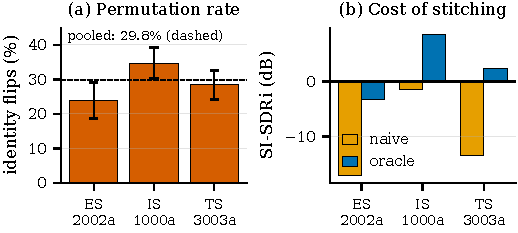
\includegraphics[width=\columnwidth]{baseline_permutation.pdf}
\caption{Window-wise blind separation on AMI. (a) Fraction of window transitions whose output-to-speaker mapping changes (95\% CI). (b) SI-SDRi of naive stitching versus an oracle assignment of the identical separator output.}
\label{fig:baseline}
\end{figure}

The separator is not the bottleneck; stitching is. A TSE model avoids both identity and gain continuity problems because every window is conditioned on the same speaker cue and there is one output per speaker. This result fixed the architecture: \emph{extract one speaker at a time, conditioned on a persistent identity cue}.

A second finding shaped the visual front end. A placeholder active-speaker detector based on lip-region motion energy, evaluated on AMI close-up video against headset activity, showed no diagonal structure in its face-to-voice agreement matrix (largest value 0.080). In the process we found that AMI's camera-to-headset mapping cannot be assumed: only 53 of about 171 meetings follow the naive \texttt{Closeup}$_{n+1}$/\texttt{Headset}$_n$ pairing, and our builder now reads the published mapping from the corpus metadata.

% ============================================================================
\section{SEAVE: A Reliability-Gated Extractor}
\label{sec:seave}
% ============================================================================

\begin{figure}[t]
\centering
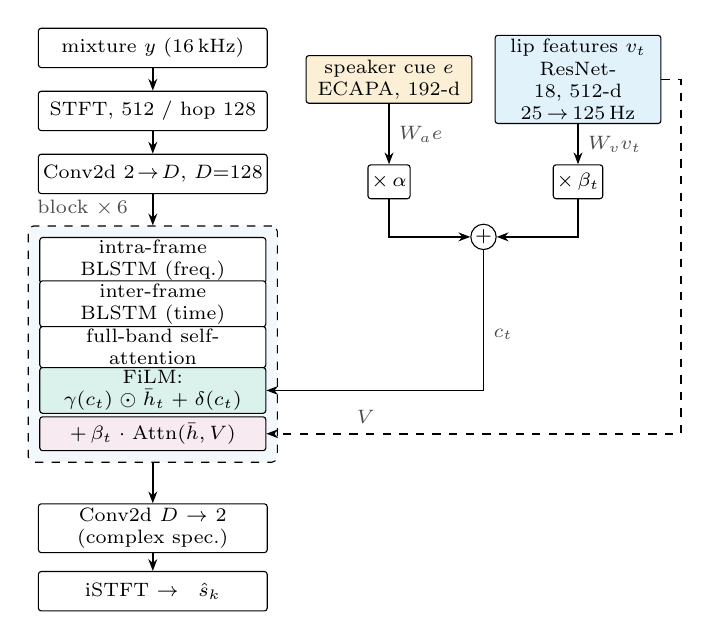
\begin{tikzpicture}[
  x=1mm, y=1mm,
  font=\scriptsize,
  box/.style={draw, rounded corners=1pt, align=center, minimum height=5mm, inner sep=1.5pt, fill=white, text width=28mm},
  sub/.style={draw, rounded corners=1pt, align=center, minimum height=4.3mm, inner sep=1pt, fill=white, text width=28mm},
  cue/.style={draw, rounded corners=1pt, align=center, inner sep=1.5pt, text width=20mm},
  gate/.style={draw, rounded corners=1pt, align=center, inner sep=1.2pt, fill=white, minimum height=4.3mm},
  op/.style={draw, circle, inner sep=0.4pt, fill=white},
  arr/.style={-{Stealth[length=1.5mm]}, semithick},
  lab/.style={font=\scriptsize, text=black!70}
]
% ---- audio path, top to bottom (x = 0) ----
\node[box] (y) at (0,0) {mixture $y$ (16\,kHz)};
\node[box] (stft) at (0,-8) {STFT, 512 / hop 128};
\node[box] (enc) at (0,-16) {Conv2d $2\!\rightarrow\!D$, $D{=}128$};
\node[sub] (intra) at (0,-27) {intra-frame BLSTM (freq.)};
\node[sub] (inter) at (0,-32.5) {inter-frame BLSTM (time)};
\node[sub] (mhsa) at (0,-38) {full-band self-attention};
\node[sub, fill=cgreen!14] (film) at (0,-43.5) {FiLM: $\gamma(c_t)\odot\bar{h}_t+\delta(c_t)$};
\node[sub, fill=cpurple!16] (xatt) at (0,-49) {$+\,\beta_t\cdot\mathrm{Attn}(\bar{h},V)$};
\begin{scope}[on background layer]
\node[draw, dashed, rounded corners=2pt, fill=cblue!5, inner sep=1.4mm, fit=(intra)(xatt)] (blk) {};
\end{scope}
\node[lab, anchor=south west] at (blk.north west) {block $\times\,6$};
\node[box] (dec) at (0,-61) {Conv2d $D\!\rightarrow\!2$ (complex spec.)};
\node[box] (istft) at (0,-69) {iSTFT $\rightarrow\ \hat{s}_k$};
\draw[arr] (y) -- (stft);
\draw[arr] (stft) -- (enc);
\draw[arr] (enc) -- (blk);
\draw[arr] (blk) -- (dec);
\draw[arr] (dec) -- (istft);
% ---- conditioning, side by side on the right ----
\node[cue, fill=corange!16] (e) at (30,-4) {speaker cue $e$\\ECAPA, 192-d};
\node[cue, fill=csky!18] (v) at (54,-4) {lip features $v_t$\\ResNet-18, 512-d\\25$\,\rightarrow\,$125\,Hz};
\node[gate] (ga) at (30,-17) {$\times\,\alpha$};
\node[gate] (gv) at (54,-17) {$\times\,\beta_t$};
\node[op] (sum) at (42,-24) {$+$};
\draw[arr] (e) -- node[lab, right] {$W_a e$} (ga);
\draw[arr] (v) -- node[lab, right] {$W_v v_t$} (gv);
\draw[arr] (ga) |- (sum);
\draw[arr] (gv) |- (sum);
\draw[arr] (sum) |- node[lab, pos=0.3, right] {$c_t$} (film.east);
\draw[arr, dashed] (v.east) -- ++(2.5,0) |- node[lab, pos=0.88, above] {$V$} (xatt.east);
\end{tikzpicture}
\caption{SEAVE. Six TF-GridNet-style blocks map the mixture spectrogram directly to the target's. A conditioning vector $c_t$ mixes a speaker embedding and lip features through learned reliability gates $\alpha$ (per utterance) and $\beta_t$ (per frame) and modulates every block by FiLM; $\beta_t$ also scales a cross-attention from audio to visual features $V$.}
\label{fig:seave}
\end{figure}

\subsection{Architecture}
SEAVE (Fig.~\ref{fig:seave}) follows TF-GridNet~\cite{wang2023tfgridnet}. The mixture is transformed by an STFT (512-point Hann window, hop 128, 16\,kHz; 257 bins at 125 frames/s), real and imaginary parts are stacked, and a $3{\times}3$ convolution embeds them into $H\in\mathbb{R}^{D\times T\times F}$ with $D=128$. Each of six blocks applies, with residual connections,
\begin{align}
H &\leftarrow H + P_f\big(\mathrm{BLSTM}_f(\mathrm{GN}(H))\big), \label{eq:intra}\\
H &\leftarrow H + P_t\big(\mathrm{BLSTM}_t(\mathrm{GN}(H))\big), \label{eq:inter}\\
H &\leftarrow H + \mathrm{MHSA}\big(\mathrm{LN}(\bar{H})\big)\otimes \mathbf{1}_F, \label{eq:attn}
\end{align}
where $\mathrm{BLSTM}_f$ runs across frequency at each frame, $\mathrm{BLSTM}_t$ across time at each frequency~\cite{hochreiter1997lstm}, $\bar{H}=\frac{1}{F}\sum_f H_{:,:,f}$ is the frequency-pooled sequence and MHSA is four-head self-attention~\cite{vaswani2017attention}. The inter-frame path is the reason for the backbone: speaker identity is a long-horizon property, and a model without such a path must re-decide whom it follows at every frame.

\subsection{Reliability-gated conditioning}
Real uploads contain head turns, occlusions and off-screen speakers; a visual cue that is wrong for two seconds should be ignored for those two seconds only. Given a speaker embedding $e\in\mathbb{R}^{192}$ with confidence $\rho_a$ and per-frame visual features $v_t\in\mathbb{R}^{512}$ with confidences $\rho_{v,t}$,
\begin{align}
\alpha &= \sigma\big(g_a(\rho_a)\big), \qquad \beta_t = \sigma\big(g_v(\rho_{v,t})\big), \label{eq:gates}\\
c_t &= \alpha\,W_a e + \beta_t\,W_v v_t + b, \label{eq:cond}
\end{align}
where $g_a,g_v$ are small learned maps (1--16--1, SiLU) and $c_t\in\mathbb{R}^{256}$. After each block the pooled features are modulated by FiLM~\cite{perez2018film}, $m_t=\gamma(c_t)\odot\bar{h}_t+\delta(c_t)$, initialised to the identity; when video is present, $m_t \leftarrow m_t + \beta_t\,\mathrm{Attn}(\mathrm{LN}(m_t), V, V)$, so the gate scales the attention \emph{output} and removes an unreliable visual contribution rather than merely redistributing attention. The change $m_t-\bar{h}_t$ is broadcast back over frequency. Conditioning at every block rather than once at the input counters dilution of the speaker request through depth. A decoder convolution produces the complex spectrogram of the target directly (no mask), followed by an inverse STFT; a small head predicts an utterance-level confidence. The model has 5.02\,M parameters; the visual front end (a 3D convolution over five frames followed by a ResNet-18~\cite{he2016resnet} trunk on $96{\times}96$ grayscale lip crops, 512-d at 25\,fps) adds 11.46\,M.

During audio-visual training, modality dropout zeroes or corrupts each cue per item (visual drop 0.20, audio-cue drop 0.15, visual corruption 0.25, audio-cue corruption 0.15) and lowers its confidence accordingly, so that the gates learn to recognise an unreliable cue rather than being told.

\subsection{Suppression-first objective}
SI-SDR penalises all error equally, but residual interference (another person talking) is far more objectionable to a listener than mild artefacts. The loss combines
\begin{equation}
\mathcal{L} = \mathcal{L}_{\sisdr} + 0.5\,\mathcal{L}_{\mathrm{sup}} + 0.2\,\mathcal{L}_{\mathrm{cons}} + 0.3\,\mathcal{L}_{\mathrm{MR}} + 0.5\,\mathcal{L}_{\mathrm{sil}},
\label{eq:loss}
\end{equation}
with $\mathcal{L}_{\sisdr}=-\sisdr(\hat{s},s)$; a hinged interference penalty $\mathcal{L}_{\mathrm{sup}}=\frac{1}{J}\sum_j \max(0,\tau+\sisdr(\hat{s},s_j))$ over interferers $s_j$ with $\tau=20$\dB, which stops pushing once leakage is $\tau$\dB below the output so that it cannot be satisfied by distorting the target; a multi-resolution STFT term~\cite{yamamoto2020pwg} (FFT sizes 512, 1024, 2048; spectral convergence plus log-magnitude $\ell_1$); and a silence term
\begin{equation}
\mathcal{L}_{\mathrm{sil}} = \frac{\mathbb{E}_{t\notin\mathcal{A}}[\,\lVert\hat{s}_t\rVert^2]}{\mathbb{E}_{t\in\mathcal{A}}[\,\lVert\hat{s}_t\rVert^2]},
\label{eq:silence}
\end{equation}
the output energy in frames where the target is inactive relative to frames where it is active ($\mathcal{A}$), which targets the 50--70\% of a conversation in which each speaker is silent and leakage is unmasked. The speaker-consistency term $\mathcal{L}_{\mathrm{cons}}$ (cosine distance between embeddings of output and enrolment) is implemented but was inactive in every run reported here, as the training logs show it at zero; we therefore make no claim about it.

\subsection{Curriculum}
\label{sec:curriculum}
Training proceeded in stages, each initialised from the last (Table~\ref{tab:training}). C1 learns separation on Libri2Mix~\cite{cosentino2020librimix} (16\,kHz, \textit{min}, train-100 and train-360 of LibriSpeech~\cite{panayotov2015librispeech}) with WHAM! noise~\cite{wichern2019wham} introduced partway through. C3 keeps the speakers and objective but builds realistic mixtures: image-source~\cite{allen1979image} room responses via pyroomacoustics~\cite{scheibler2018pyroomacoustics} (rooms $3{\times}3{\times}2.4$ to $10{\times}8{\times}3.5$\,m, RT60 log-uniform in 0.15--0.8\,s, reflection order 12), turn-taking rather than uniform overlap, per-speaker level spread, noise at 5--25\dB SNR, and a lossy codec round trip half the time. C2 adds the visual path on VoxCeleb2~\cite{chung2018voxceleb2} audio-visual mixtures built from the 118-speaker test split with speaker-disjoint validation. All stages use AdamW~\cite{loshchilov2019adamw} (weight decay 0.01), linear warm-up for 500 steps then cosine decay, gradient clipping at 5, bf16 autocast and gradient checkpointing~\cite{chen2016checkpoint}, on one NVIDIA RTX A5000 (24\,GB). A dataloader benchmark sustained 295 items/s and 97.5\% GPU utilisation for a realistically sized model.

\begin{table}[t]
\centering
\caption{Training stages (values read from the checkpoints and run logs)}
\label{tab:training}
\setlength{\tabcolsep}{3.2pt}
\begin{tabular}{@{}lllrrr@{}}
\toprule
Stage & Data & Init. & Steps & LR & Best val. \\
\midrule
C1 & Libri2Mix + WHAM! & --- & 60k & $1.5{\times}10^{-4}$ & 8.34\dB$^a$ \\
C3 & + room simulation & C1 & 30k & $8{\times}10^{-5}$ & 10.92\dB$^b$ \\
C2 v2 & VoxCeleb2 AV & C3 & 12k & $6{\times}10^{-5}$ & 11.43\dB$^c$ \\
\bottomrule
\multicolumn{6}{@{}p{0.95\columnwidth}@{}}{\footnotesize $^a$Libri2Mix dev. $^b$Room-simulated Libri2Mix dev. $^c$VoxCeleb2 held-out speakers, audio-visual; 11.02\dB with only the audio cue and 11.02\dB with only the visual cue at the same step.}
\end{tabular}
\end{table}

% ============================================================================
\section{The VisioVox System}
\label{sec:system}
% ============================================================================

\begin{figure*}[t]
\centering
\resizebox{\textwidth}{!}{%
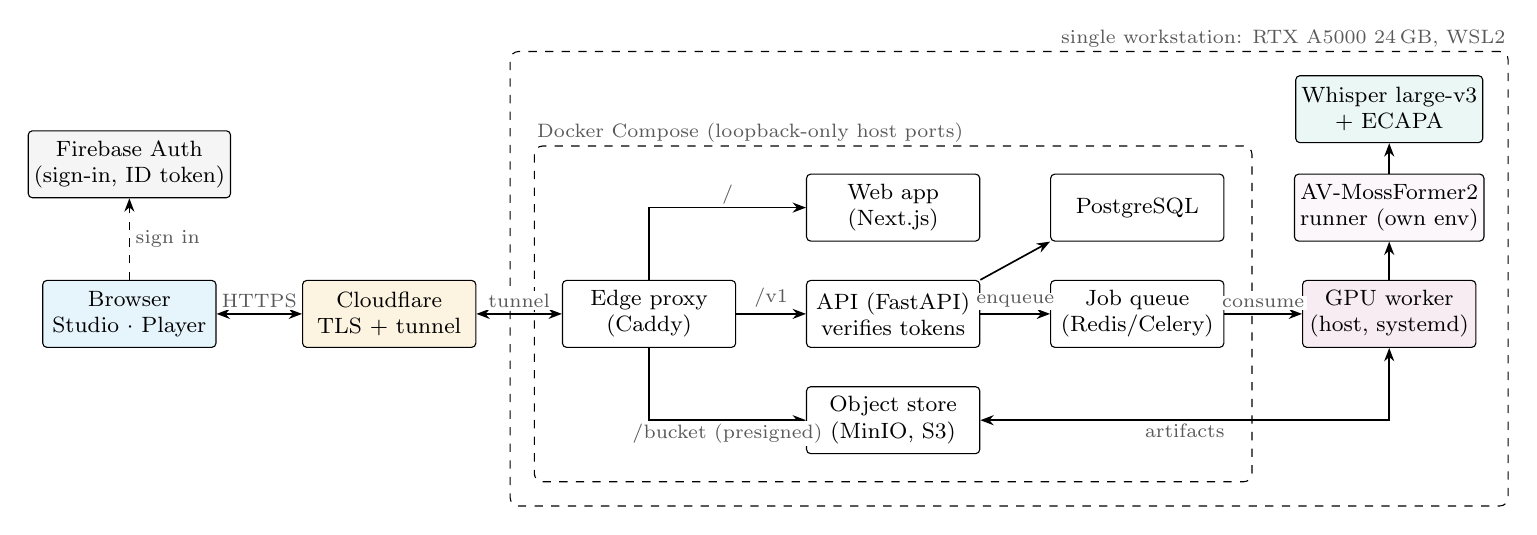
\begin{tikzpicture}[
  font=\footnotesize,
  box/.style={draw, rounded corners=1.5pt, align=center, minimum height=8.5mm, minimum width=22mm, inner sep=2pt, fill=white},
  arr/.style={-{Stealth[length=1.7mm]}, semithick},
  darr/.style={{Stealth[length=1.7mm]}-{Stealth[length=1.7mm]}, semithick},
  grp/.style={draw, dashed, rounded corners=3pt},
  lab/.style={font=\scriptsize, text=black!65, align=center, fill=white, inner sep=1pt}
]
\node[box, fill=csky!15] (browser) at (0,0) {Browser\\Studio $\cdot$ Player};
\node[box, fill=black!4] (fb) at (0,1.9) {Firebase Auth\\(sign-in, ID token)};
\node[box, fill=corange!12] (cf) at (3.3,0) {Cloudflare\\TLS + tunnel};
\node[box] (edge) at (6.6,0) {Edge proxy\\(Caddy)};
\node[box] (web) at (9.7,1.35) {Web app\\(Next.js)};
\node[box] (api) at (9.7,0) {API (FastAPI)\\verifies tokens};
\node[box] (minio) at (9.7,-1.35) {Object store\\(MinIO, S3)};
\node[box] (redis) at (12.8,0) {Job queue\\(Redis/Celery)};
\node[box] (pg) at (12.8,1.35) {PostgreSQL};
\node[box, fill=cpurple!14] (worker) at (16.0,0) {GPU worker\\(host, systemd)};
\node[box, fill=cpurple!6] (tse) at (16.0,1.35) {AV-MossFormer2\\runner (own env)};
\node[box, fill=cgreen!8] (asr) at (16.0,2.6) {Whisper large-v3\\+ ECAPA};

\begin{scope}[on background layer]
\node[grp, fit=(edge)(web)(api)(minio)(redis)(pg), inner sep=3.5mm] (compose) {};
\node[grp, fit=(compose)(worker)(tse)(asr), inner sep=3mm] (host) {};
\end{scope}
\node[lab, anchor=south west, fill=none] at (compose.north west) {Docker Compose (loopback-only host ports)};
\node[lab, anchor=south east, fill=none] at (host.north east) {single workstation: RTX A5000 24\,GB, WSL2};

\draw[darr] (browser) -- node[lab, above=1pt] {HTTPS} (cf);
\draw[darr] (cf) -- node[lab, above=1pt] {tunnel} (edge);
\draw[arr] (edge.north) |- node[lab, pos=0.75, above] {/} (web.west);
\draw[arr] (edge) -- node[lab, above=1pt] {/v1} (api);
\draw[arr] (edge.south) |- node[lab, pos=0.75, below] {/bucket (presigned)} (minio.west);
\draw[arr] (api) -- node[lab, above=1pt] {enqueue} (redis);
\draw[arr] (api.north east) -- (pg.south west);
\draw[arr] (redis) -- node[lab, above=1pt] {consume} (worker);
\draw[arr] (worker) -- (tse);
\draw[arr] (tse) -- (asr);
\draw[darr] (worker.south) |- node[lab, pos=0.75, below] {artifacts} (minio.east);
\draw[arr, dashed] (browser) -- node[lab, right=1pt] {sign in} (fb);
\end{tikzpicture}}
\caption{Deployment. Every component runs on one workstation. The browser reaches a single public origin through a Cloudflare tunnel; an edge proxy routes \texttt{/v1} to the API, the bucket path to the object store (uploads and playback use URLs presigned for the public host) and everything else to the web app. The API verifies Firebase ID tokens and enqueues jobs by task name; the GPU worker runs on the host and reaches the data services on loopback ports.}
\label{fig:arch}
\end{figure*}

\subsection{Overview and deployment}
Fig.~\ref{fig:arch} shows the deployed system. Recurring cost is zero: the workstation that trained the models serves them, a Cloudflare tunnel provides HTTPS without a public IP or open port, the domain is a free subdomain, and authentication uses Firebase's free tier. Uploads go from the browser directly to the S3-compatible object store via multipart presigned URLs (16\,MiB parts, resumable). Because SigV4 signs the \texttt{Host} header, URLs are signed for the public origin and the edge proxy forwards that host unchanged. The API never imports worker code; it sends jobs by task name, and a GPU worker with concurrency one consumes them, so a second upload queues rather than contending for GPU memory.

\subsection{Processing pipeline}
The serving pipeline (Fig.~\ref{fig:pipeline}) replaced SEAVE with AV-MossFormer2~\cite{clearervoice} for the reasons discussed in Section~\ref{sec:discussion}. Its stages are:

\begin{figure}[t]
\centering
\resizebox{\columnwidth}{!}{%
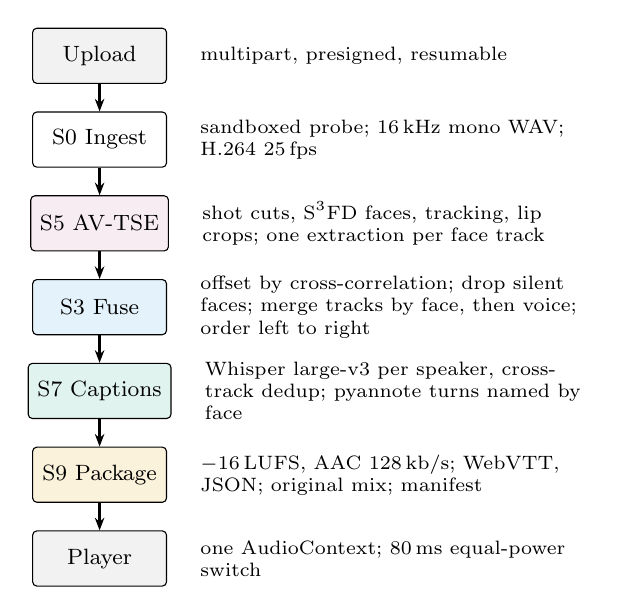
\begin{tikzpicture}[
  font=\footnotesize,
  st/.style={draw, rounded corners=1.5pt, minimum width=17mm, minimum height=7mm, align=center, fill=white},
  note/.style={font=\scriptsize, align=left, text width=50mm, anchor=west},
  arr/.style={-{Stealth[length=1.6mm]}, thick}
]
\node[st, fill=black!5] (up) {Upload};
\node[st, below=3.5mm of up] (s0) {S0 Ingest};
\node[st, below=3.5mm of s0, fill=cpurple!14] (s5) {S5 AV-TSE};
\node[st, below=3.5mm of s5, fill=csky!16] (s3) {S3 Fuse};
\node[st, below=3.5mm of s3, fill=cgreen!12] (s7) {S7 Captions};
\node[st, below=3.5mm of s7, fill=corange!14] (s9) {S9 Package};
\node[st, below=3.5mm of s9, fill=black!5] (pl) {Player};
\foreach \a/\b in {up/s0, s0/s5, s5/s3, s3/s7, s7/s9, s9/pl} \draw[arr] (\a) -- (\b);
\node[note, right=3mm of up] {multipart, presigned, resumable};
\node[note, right=3mm of s0] {sandboxed probe; 16\,kHz mono WAV; H.264 25\,fps};
\node[note, right=3mm of s5] {shot cuts, S$^3$FD faces, tracking, lip crops; one extraction per face track};
\node[note, right=3mm of s3] {offset by cross-correlation; drop silent faces; merge tracks by face, then voice; order left to right};
\node[note, right=3mm of s7] {Whisper large-v3 per speaker, cross-track dedup; pyannote turns named by face};
\node[note, right=3mm of s9] {$-16$\,LUFS, AAC 128\,kb/s; WebVTT, JSON; original mix; manifest};
\node[note, right=3mm of pl] {one AudioContext; 80\,ms equal-power switch};
\end{tikzpicture}}
\caption{Serving pipeline. A speaker is a face track: the extractor is conditioned on lip movement, and S3 turns per-track outputs into one full-length track per person.}
\label{fig:pipeline}
\end{figure}

\textbf{S0 Ingest.} The upload is probed in a sandbox before any decoding and normalised into a 16\,kHz mono analysis WAV and a constant-25\,fps H.264 video (8-bit 4:2:0 with the index first, so the same file is browser-playable). An upload without video is refused with an explanation, since the extractor requires faces.

\textbf{S5 Audio-visual extraction.} A separate process in the extractor's own environment detects shot boundaries, runs the S$^3$FD face detector~\cite{zhang2017s3fd} on every frame, links detections into face tracks, crops lip regions and runs AV-MossFormer2 once per track over that track's span of the analysis WAV. It returns, per track $i$, its frame span $[f_i^{s}, f_i^{e})$, mean horizontal position and the separated waveform $\hat{s}_i$.

\textbf{S3 Fusion: from face tracks to people.} Per-track outputs cover only the frames in which a face was visible and are counted on the extractor's own re-encoded timeline. Let $a$ be the analysis waveform and $r$ the extractor's input waveform. The container offset is estimated, never assumed, as
\begin{equation}
\ell^{*} = \arg\max_{|\ell|\le L}\Big|\sum_{t} r(t+\ell)\,a(t)\Big|,
\label{eq:lag}
\end{equation}
over the first 60\,s with $L$ = 1\,s, and track $i$ is placed at sample $640 f_i^{s}-\ell^{*}$ on a zero-initialised full-length buffer (640 samples per video frame at 16\,kHz). We observed $\ell^{*}=1105$ samples (69.1\,ms) when the extractor's audio came from an AAC container and $\ell^{*}=0$ once it was fed the analysis WAV directly. A track is discarded as a non-speaking face if
\begin{equation}
20\log_{10}\frac{\mathrm{RMS}(\hat{s}_i[\mathcal{T}_i])}{\mathrm{RMS}(a[\mathcal{T}_i])} < -30\,\mathrm{dB},
\label{eq:silent}
\end{equation}
over its span $\mathcal{T}_i$. A camera cut or lost detection splits one person into several tracks, so tracks that never overlap in time are merged when their faces match---ArcFace~\cite{deng2019arcface} embeddings averaged over eight frames of the extractor's own crops, $\cos(f_i,f_j)>0.3$---or, where no face can be embedded, when ECAPA~\cite{desplanques2020ecapa} embeddings of their active speech satisfy $\cos(e_i,e_j)>0.6$; tracks that overlap in time are never merged, since one face cannot be on screen twice. The face cue was added after Section~\ref{sec:amiav} showed voice alone splitting people. Speakers are numbered left to right. The extractor reports no confidence, so each speaker is labelled with the fraction of the recording in which its face was tracked---an upper bound on how complete its track can be. The overlap ratio shown to the user is measured on the separated tracks as the share of active frames (energy above $-30$\dB relative to the track's 95th-percentile frame) in which two or more speakers are active.

\textbf{S7 Captions.} Each separated track is transcribed by Whisper large-v3~\cite{radford2023whisper} (faster-whisper~\cite{fasterwhisper}, float16, Silero VAD, no conditioning on previous text) with word timestamps, so captions reflect what was recovered. Because every track also carries the other speakers a few decibels down and Whisper transcribes them, words that recur across tracks at the same moment are then kept only in the track that retains most of their energy (Section~\ref{sec:amiav}). The same stage diarizes the mixture and names each diarized speaker by face (Section~\ref{sec:conversation}); the resulting speaking intervals ride in each speaker's caption file, so a failure here costs the conversation insights their best timing, never the job.

\textbf{S9 Packaging and playback.} Tracks are loudness-normalised to $-16$\,LUFS (ITU-R BS.1770~\cite{itu1770}), encoded as AAC, and shipped with WebVTT~\cite{webvtt} and word-level JSON captions, the unprocessed mixture as an ``original mix'' track, the video, and a manifest. The player decodes all tracks into one Web Audio~\cite{webaudio} context and switches speakers with an 80\,ms equal-power crossfade. Audio-video drift below 40\,ms is left alone, drift between 40 and 250\,ms is removed by trimming the playback rate by at most 0.4\%, and larger jumps re-anchor the clocks; the active speaker's captions are highlighted word by word (Fig.~\ref{fig:ui}). Projects longer than 10\,min or with more than four tracks are flagged for HLS~\cite{rfc8216}.

\begin{figure}[t]
\centering
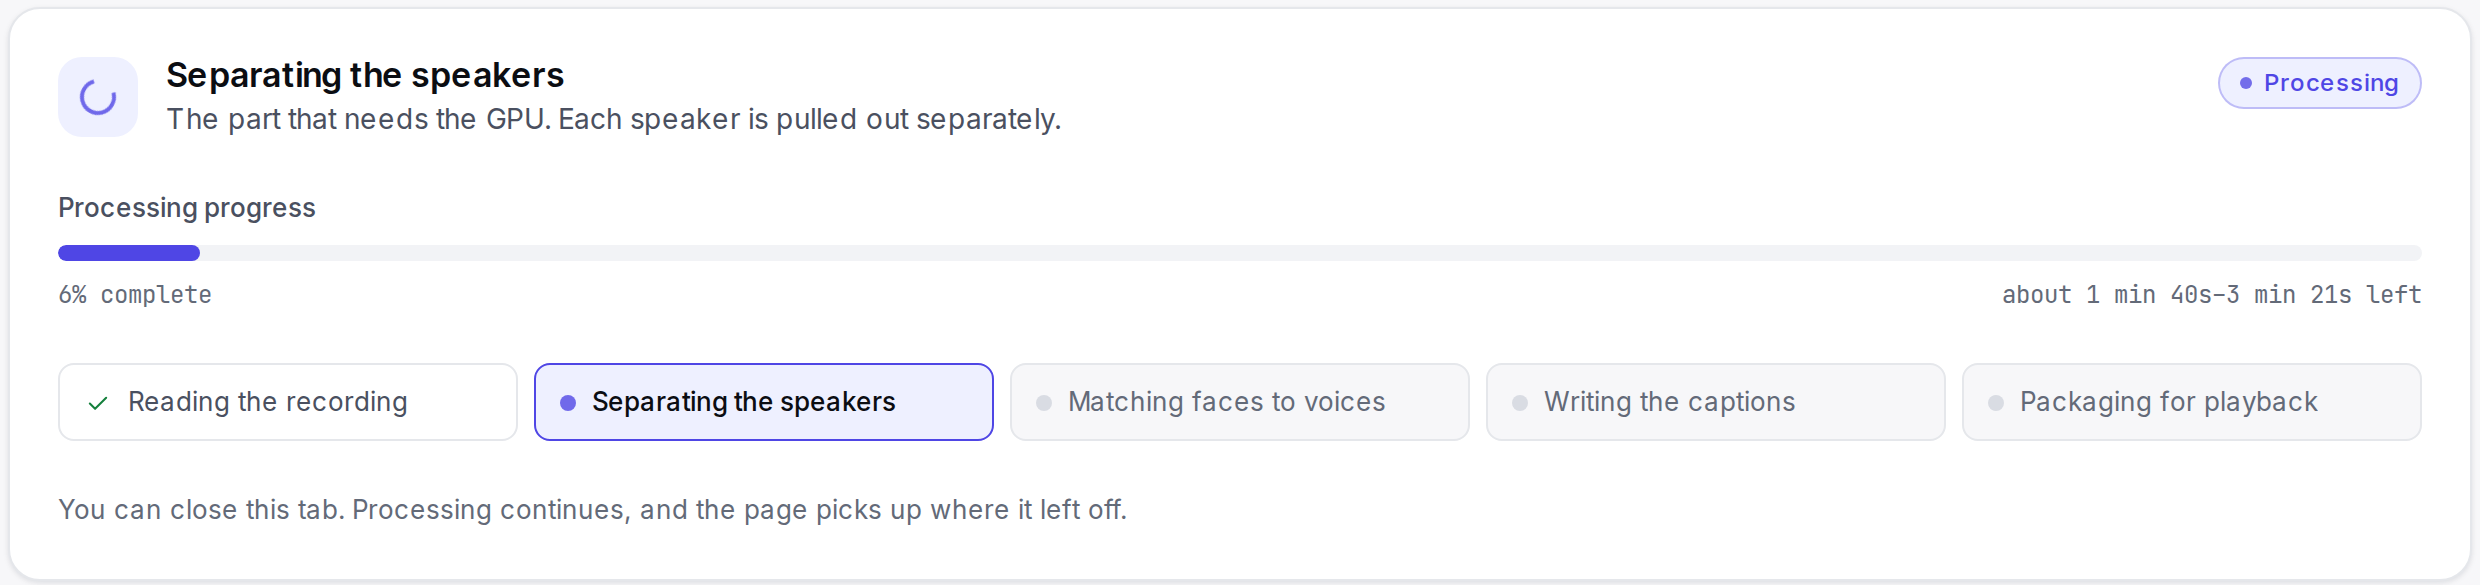
\includegraphics[width=0.97\columnwidth]{ui_studio.png}\\[1mm]
\footnotesize (a) Processing\\[1.5mm]
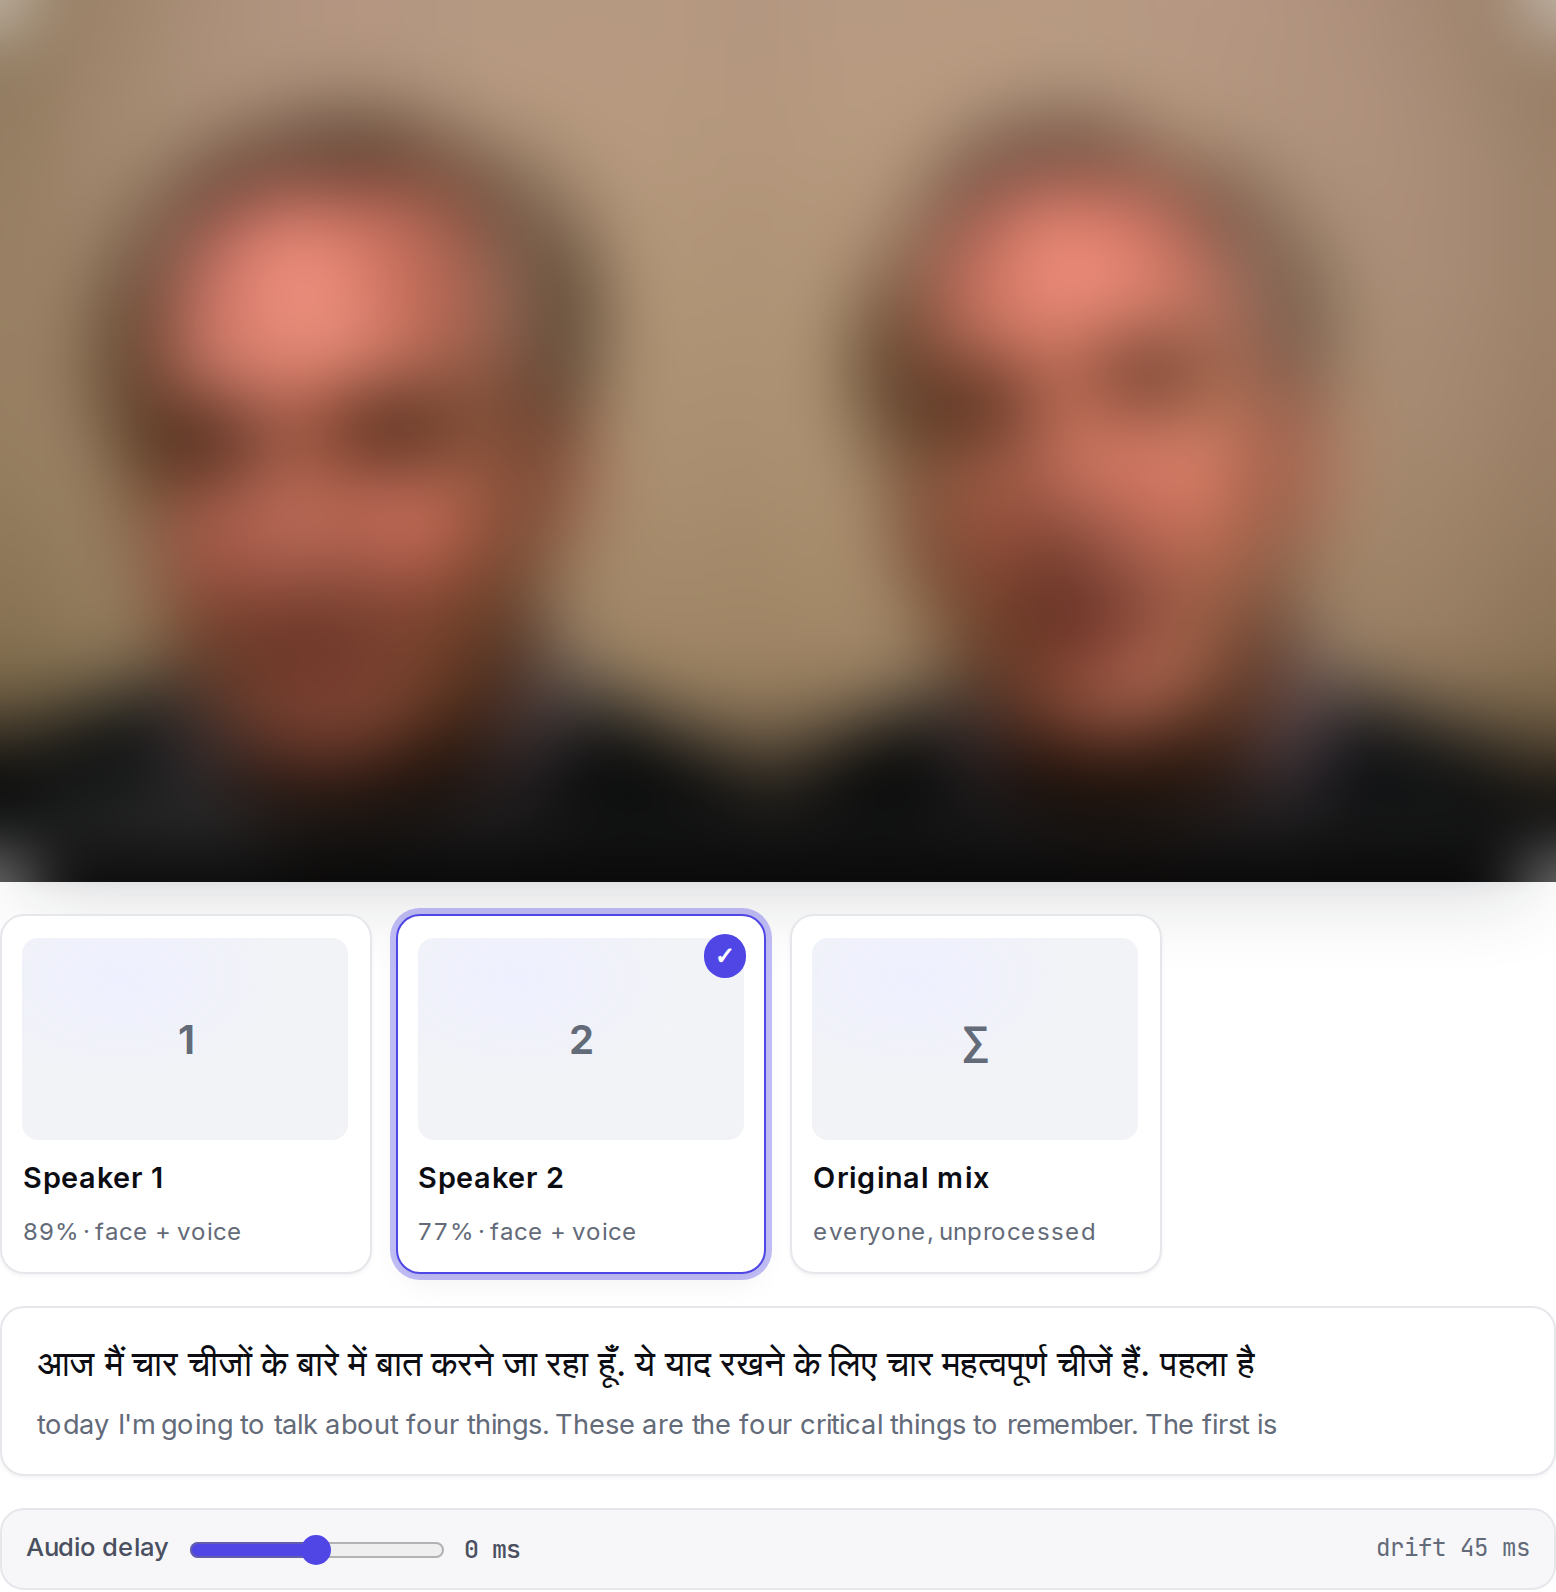
\includegraphics[width=0.72\columnwidth]{ui_player.png}\\[1mm]
\footnotesize (b) Player, speaker~2 selected (video blurred for this paper)
\caption{Production interface, captured at 2$\times$ by the end-to-end browser test. (a) The current stage, progress, a time estimate from measured real-time factors, and the five steps the pipeline actually runs. (b) Per-speaker tracks with tracked-face coverage, the original mix, and the selected speaker's caption, here machine-translated into Hindi with the words as spoken beneath.}
\label{fig:ui}
\end{figure}

\textbf{Communicating progress.} Processing takes tens of seconds to minutes, so the interface names the stage the pipeline is in (reading the recording, separating the speakers, matching faces to voices, writing the captions, packaging for playback), shows its progress and a time range from the measured real-time factors, and drives every element from one state model; nothing advances on a timer (Fig.~\ref{fig:ui}a). Progress arrives over server-sent events with a polling fallback, and the page resumes where it was if closed.

% ============================================================================
\section{Experiments and Results}
\label{sec:results}
% ============================================================================

\subsection{Training behaviour}
Fig.~\ref{fig:training} shows validation SI-SDRi during each stage. C1 reached 8.34\dB on Libri2Mix dev. C3, initialised from C1 and evaluated on room-simulated dev mixtures (a harder distribution), reached 10.92\dB at step 27k. On VoxCeleb2, C2 v2 reached 11.43\dB with both cues; the audio-only and visual-only paths reached 11.02\dB each, so on this data the visual cue added about 0.4\dB over the voice embedding alone.

\begin{figure*}[t]
\centering
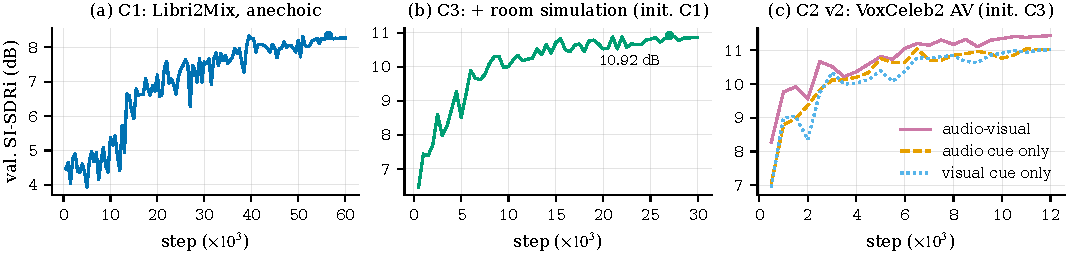
\includegraphics[width=\textwidth]{training_curves.pdf}
\caption{Validation SI-SDRi during training. Each stage is validated on its own development data, so the panels are not on a common scale.}
\label{fig:training}
\end{figure*}

\subsection{Product-condition evaluation}
Each validation set in Fig.~\ref{fig:training} measures something adjacent to the deployed task. Libri2Mix has overlap but no room; AMI has rooms, but measured properly contains little simultaneous speech (across ten meetings, one 4\,s window had two people both clearly talking), so averaging over it scores a separator on audio that needs no separation. We therefore built the condition directly: real speech from Libri2Mix dev, simulated rooms with the C3 simulator, a requested overlap of 30--70\%, and items discarded unless the overlap measured on the reverberant sources is at least 25\%. Items are generated from a fixed seed, so every model sees identical mixtures (181 two-speaker and 200 three-speaker items; measured overlap 31\% and 36\%; mixture SI-SDR $+0.36$ and $-3.99$\dB). Confidence intervals are bootstrap 95\% intervals~\cite{efron1993bootstrap}. The test is audio-only, so the audio-visual models are evaluated through their audio-cue path.

\begin{table}[t]
\centering
\caption{SI-SDRi (dB) on the product condition}
\label{tab:product}
\setlength{\tabcolsep}{2.2pt}
\footnotesize
\begin{tabular}{@{}llrcrc@{}}
\toprule
 & & \multicolumn{2}{c}{2 speakers ($n$=181)} & \multicolumn{2}{c}{3 speakers ($n$=200)} \\
\cmidrule(lr){3-4}\cmidrule(l){5-6}
Model & Data & SI-SDRi & 95\% CI & SI-SDRi & 95\% CI \\
\midrule
C1 & Libri2Mix & $-2.09$ & $[-3.53, -0.70]$ & $-0.81$ & $[-2.16, 0.41]$ \\
C3 & + room sim. & $\mathbf{+8.25}$ & $[7.41, 9.14]$ & $\mathbf{+6.34}$ & $[5.39, 7.20]$ \\
C2 v1 & VoxCeleb2, 8k & $+2.49$ & $[1.17, 3.68]$ & $+0.75$ & $[-0.61, 2.03]$ \\
C2 v2 & VoxCeleb2, 12k & $-1.61$ & $[-4.06, 0.73]$ & $-0.97$ & $[-2.74, 0.79]$ \\
\midrule
\multicolumn{2}{@{}l}{Mixture SI-SDR (input)} & $+0.36$ & & $-3.99$ & \\
\bottomrule
\end{tabular}

\end{table}

\begin{figure*}[t]
\centering
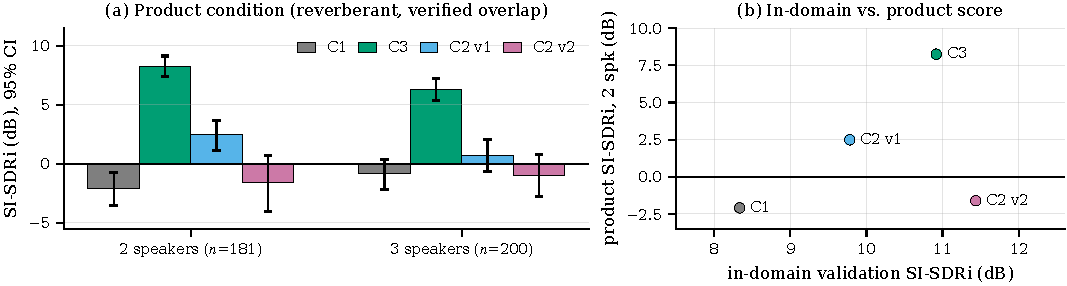
\includegraphics[width=\textwidth]{product_condition.pdf}
\caption{(a) SI-SDRi on the product condition (bootstrap 95\% CI). (b) Each model's best in-domain validation score against its two-speaker product score: the ordering is not preserved.}
\label{fig:product}
\end{figure*}

Table~\ref{tab:product} and Fig.~\ref{fig:product} show the result. C3 is the only model that holds up: $+8.25$\dB (95\% CI [7.41, 9.14]) with two speakers and $+6.34$\dB with three. The checkpoint with the best in-domain score, C2 v2 ($+11.43$\dB on VoxCeleb2), scores $-1.61$\dB---it makes the audio worse than doing nothing---and the anechoic C1 scores $-2.09$\dB. C2 v1, trained for fewer steps on VoxCeleb2, falls in between ($+2.49$\dB). The pattern is a dose-response: the further a model trains on data without room acoustics, the more of the robustness learned in C3 it loses, and its in-domain score rises while it does so. Model selection on in-domain validation would have shipped the worst model. A further run, C2 v3, therefore blends room-simulated LibriMix into half of the micro-batches and selects the checkpoint maximising the minimum of its in-domain and product-validation scores (step 4.5k; 10.37\dB in-domain). It recovers most of the loss: $+6.71$\dB [5.55, 7.78] with two speakers and $+4.92$\dB with three, against $-1.61$ and $-0.97$\dB for C2 v2, though still below C3. Its final checkpoint scores higher here ($+7.28$\dB) but was not the one selected, so it is not reported as the result.

\subsection{Deployed extractor on overlapped video}
Because the product condition is audio-only, it cannot assess a lip-driven extractor. As a first audio-visual check we built three 6\,s test videos, each placing two different VoxCeleb2 test-set speakers side by side (224$\times$224 per face) over a mixture at 0\dB relative level with full overlap, and ran AV-MossFormer2 through the S5 runner. Table~\ref{tab:moss} reports the six extracted tracks after the container offset was removed: mean SI-SDRi $+9.43$\dB (range $+5.67$ to $+12.57$), with each output at $-18$ to $-34$\dB SI-SDR against the other speaker, i.e., the correct person was extracted every time. This is a small, favourable test and is not comparable with Table~\ref{tab:product}; Section~\ref{sec:amiav} evaluates the same extractor on real meetings.

\begin{table}[t]
\centering
\caption{AV-MossFormer2 on synthetic two-face overlapped videos (SI-SDR, dB). ``Leak'' is SI-SDR of the output against the other speaker.}
\label{tab:moss}
\footnotesize
\setlength{\tabcolsep}{4pt}
\begin{tabular}{@{}llrrrr@{}}
\toprule
Pair & Side & Mix & Output & SI-SDRi & Leak \\
\midrule
P1 & left & $+0.06$ & $+7.75$ & $+7.70$ & $-18.1$ \\
P1 & right & $+0.06$ & $+5.73$ & $+5.67$ & $-30.4$ \\
P2 & left & $-0.09$ & $+12.48$ & $+12.57$ & $-34.1$ \\
P2 & right & $-0.09$ & $+10.78$ & $+10.86$ & $-31.3$ \\
P3 & left & $+0.17$ & $+10.41$ & $+10.24$ & $-25.4$ \\
P3 & right & $+0.17$ & $+9.74$ & $+9.56$ & $-26.8$ \\
\midrule
Mean & & & & $\mathbf{+9.43}$ & \\
\bottomrule
\end{tabular}

\end{table}

\subsection{Latency in production}
Fig.~\ref{fig:latency} and Table~\ref{tab:latency} report all 24 successful jobs processed by the deployed system during development and acceptance testing: seven distinct videos of 6.0--32.2\,s, from 448$\times$224 to 1920$\times$3414, every one yielding two speakers. The median real-time factor (job time over video duration) was 2.62 (mean 3.38, range 1.81--8.17). The AV-TSE stage accounted for 72\% of job time on average. High-resolution phone videos (1080p and above) ran at a real-time factor of 5.4--8.0, against 2.1--4.0 for videos of 1280$\times$720 or below, where the highest value belongs to the shortest (6\,s) clip and reflects fixed per-job cost; S5 runs face detection on every frame at the source resolution, which we expect to account for most of this difference, although its share of S5 was not measured separately. Captioning took 3--27\,s per job.

\begin{figure*}[t]
\centering
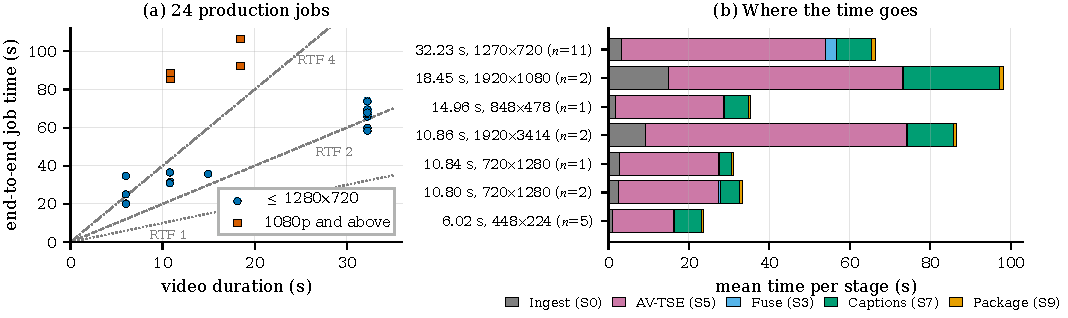
\includegraphics[width=\textwidth]{latency.pdf}
\caption{Production latency. (a) End-to-end job time against video duration for 24 jobs, with real-time-factor guides. (b) Mean time per stage for each distinct video.}
\label{fig:latency}
\end{figure*}

\begin{table}[t]
\centering
\caption{Production jobs: mean stage and total times}
\label{tab:latency}
\setlength{\tabcolsep}{3.4pt}
\footnotesize
\begin{tabular}{@{}rrrrrrr@{}}
\toprule
Dur. (s) & Resolution & $n$ & S5 (s) & S7 (s) & Total (s) & RTF \\
\midrule
6.02 & 448$\times$224 & 5 & 15.1 & 6.8 & 24.0 & 3.99 \\
10.80 & 720$\times$1280 & 2 & 24.9 & 4.8 & 33.7 & 3.12 \\
10.84 & 720$\times$1280 & 1 & 24.7 & 2.9 & 31.6 & 2.91 \\
10.86 & 1920$\times$3414 & 2 & 64.8 & 11.5 & 87.2 & 8.03 \\
14.96 & 848$\times$478 & 1 & 26.7 & 5.8 & 35.7 & 2.39 \\
18.45 & 1920$\times$1080 & 2 & 58.1 & 23.9 & 99.2 & 5.38 \\
32.23 & 1270$\times$720 & 11 & 50.7 & 8.7 & 67.1 & 2.08 \\
\midrule
All & & 24 & & & & 3.38 \\
\bottomrule
\end{tabular}

\end{table}

% ============================================================================
\section{Real Meetings: the AMI-AV Evaluation}
\label{sec:amiav}
% ============================================================================

Table~\ref{tab:moss} tests whether the deployed extractor follows the right lips in a favourable synthetic setting. This section measures what it, and the system around it, does on real recordings.

\subsection{Benchmark construction}
AMI~\cite{carletta2005ami} records each participant twice---a close-up camera on the face and a close-talking headset---which makes a real multi-speaker video with per-speaker ground truth possible without simulation. For each of 30 meetings we take the 120\,s window with the most simultaneous speech after the first minute, tile the four close-ups into one 2$\times$2 video (704$\times$576, 25\,fps) using AMI's published channel-to-camera mapping, and pair it with the sum of the four headsets. Ten TNO meetings (TS3003a--TS3012a) are held out; the 20 Edinburgh and Idiap meetings are used only where a parameter must be fitted. Nothing is simulated except the tiling: participants turn away, look down, walk to the whiteboard and pass in front of other cameras.

Three corrections were needed, each measured before it was made. (i)~\emph{Who is speaking} comes from AMI's hand-corrected word alignments ($\pm$50\,ms), not headset energy: some headsets sit near $-55$\,dBFS and carry the room within 5\dB of their wearer, and an energy detector reported 47\,s of speech for a participant who says nothing in the window. (ii)~\emph{Levels}: headset gains differ by up to 30\dB within a meeting, so each headset is scaled to $-26$\,dBFS active speech before summing. (iii)~\emph{References}: a headset whose level while only others speak is within 10\dB of its wearer's speech, or whose wearer speaks for under 2\,s, is not used as a signal reference (81 of 114 speakers remain). The rule was fixed before any system was scored; visibility, identity and word-error measures need no headset and use every participant. Audio-video synchrony was verified (extraction quality peaks at zero offset). Each system runs exactly as deployed, and each person it finds is assigned to a seat by where their face lies in the grid---never by which output scores best, which would hide identity errors.

\subsection{The extractor on real meetings}
Table~\ref{tab:amiav} summarises AV-MossFormer2 through stages S5 and S3 on all 30 meetings. Where the face is visible it helps on real overlapped speech: $+3.48$\dB SI-SDRi over the frames in which the speaker and someone else are both inside aligned words. But 14.4\% of all speech is spoken while the speaker's face is not tracked (20 of 114 speakers are covered for under 90\% of their speech, six never), the 120 seats yield 152 people because tracks of one person are not always merged, and when its own person is silent an output is only 3.8\dB below the mixture. Whole-clip STOI~\cite{taal2011stoi} falls from 0.65 to 0.54. PESQ is not reported: ITU-T P.862 is specified for 8--12\,s samples, not two-minute conversations.

\begin{table}[t]
\centering
\caption{AV-MossFormer2 (S5+S3) on 30 AMI-AV meetings. SI-SDRi (dB) with 95\% bootstrap intervals.}
\label{tab:amiav}
\footnotesize
\setlength{\tabcolsep}{3pt}
\begin{tabular}{@{}lr@{}}
\toprule
Measure & Value \\
\midrule
Speech while face untracked & 14.4\% of 65 min \\
Speakers $<$90\% / never covered & 20 / 6 of 114 \\
People found for 120 seats & 152 \\
Seats split into $>$1 person & 21 \\
People spanning two seats & 3 \\
Overlap SI-SDRi, face seen $\ge$90\% ($n$=65) & $+3.48$ {\scriptsize$[+2.61, +4.32]$} \\
Overlap SI-SDRi, all reliable ($n$=71) & $+1.87$ {\scriptsize$[-0.40, +3.54]$} \\
Output vs.\ mixture, own person silent (dB) & $-3.8$ {\scriptsize$[-4.6, -2.9]$} \\
STOI, output / mixture & 0.54 / 0.65 \\
\bottomrule
\end{tabular}

\end{table}

\subsection{Who said what}
Captions are what the product promises beyond audio, so they are scored against AMI's manual transcript. cpWER~\cite{watanabe2020chime6} (computed with MeetEval~\cite{vonneumann2023meeteval}) pairs each system's word streams with participants in whichever way minimises errors; it rewards a diarizer's anonymous but consistent clusters. VisioVox must put each caption under the right \emph{face}, so we also report seat-attributed WER (saWER): the stream for seat $k$ is scored against the person in seat $k$, with no free permutation. All systems use the deployed Whisper large-v3 (beam 5, Silero VAD on, no conditioning on previous text) and Whisper's English normaliser. Table~\ref{tab:captions} gives results on the ten held-out meetings.

\begin{table}[t]
\centering
\caption{Captions on the 10 held-out AMI-AV meetings: pooled WER (\%) with 95\% bootstrap intervals over meetings; Ins.\ = insertions. $^\dagger$plain WER, no speakers. $^\ddagger$equal-level close-talk headsets.}
\label{tab:captions}
\footnotesize
\setlength{\tabcolsep}{2pt}
\begin{tabular}{@{}lccr@{}}
\toprule
System & saWER (\%) & cpWER (\%) & Ins. \\
\midrule
Whisper, mixture$^\dagger$ & -- & 31.1 {\scriptsize[27.0, 34.5]} & -- \\
pyannote + Whisper & -- & 61.2 {\scriptsize[48.0, 77.0]} & 12.1 \\
Per-headset$^\ddagger$ & -- & 122.5 {\scriptsize[97.1, 147.8]} & 104.7 \\
\midrule
Per-track (before) & 110.2 {\scriptsize[93.1, 129.7]} & 96.1 {\scriptsize[87.1, 104.4]} & 57.3 \\
\textbf{+ dedup (deployed)} & 78.1 {\scriptsize[63.7, 94.4]} & 68.7 {\scriptsize[59.9, 76.7]} & 16.7 \\
\midrule
+ dedup, SEAVE fill & 78.3 {\scriptsize[63.7, 94.2]} & 69.7 {\scriptsize[59.9, 79.3]} & 19.2 \\
Transcribe once & 76.6 {\scriptsize[64.4, 90.6]} & 66.1 {\scriptsize[59.5, 73.1]} & -- \\
pyannote, by face & 90.5 {\scriptsize[77.1, 105.7]} & 75.2 {\scriptsize[63.8, 88.3]} & -- \\
\midrule
Oracle attribution & 45.1 {\scriptsize[39.3, 49.9]} & 45.1 {\scriptsize[39.3, 49.9]} & -- \\
\bottomrule
\end{tabular}

\end{table}

\textbf{Per-track transcription fails, and not because of separation quality.} Transcribing each person's track---the design deployed until this evaluation---places words under the right face with 110\% error, most of it insertions: every track keeps the room a few decibels down, and Whisper transcribes it, so each face is captioned with most of the meeting. Transcribing each \emph{close-talk headset} the same way is worse still (122.5\% cpWER, 104.7\% insertions), although bleed in those channels sits 13--25\dB below the wearer. No separator can be expected to leak less than a close-talk microphone; the remedy has to be in how words are attributed.

\textbf{Cross-track deduplication.} Cross-talk and genuine overlap leave different traces in the per-track transcripts: cross-talk is the \emph{same} word appearing in several tracks at the same moment, genuine overlap is \emph{different} words. We therefore keep every word that appears in one track only, and for a word that recurs across tracks---identical normalised text, midpoints within 0.5\,s, a rule fixed before scoring---keep only the copy in the track that retains most of the mixture's energy over it, $\arg\max_k \frac{1}{|W|}\sum_{t\in W} 10\log_{10}\bar{E}(s_k)(t)/\bar{E}(x)(t)$, with $s_k$ track $k$, $x$ the mixture, $W$ the word's frames and $\bar{E}$ short-term energy smoothed over 50\,ms (fitted on the 20 fitting meetings). On the held-out meetings this lowers saWER from 110.2\% to 78.1\% (paired difference $-32.1$ points, 95\% CI $[-39.0, -24.6]$) and cpWER to 68.7\%, statistically indistinguishable from pyannote~3.1~\cite{bredin2020pyannote,plaquet2023powerset} with Whisper on the mixture ($+7.5$ points, $[-8.8, +23.4]$). On the 20 fitting meetings pyannote is clearly better (40.4\% against 63.5\% cpWER), so we do not claim parity with audio-only diarization in general; the system's distinguishing property is that every word is bound to a visible face, which a diarizer alone cannot provide.

\textbf{Why not transcribe once?} Transcribing the mixture once and giving each word to the track that retains it is tied with deduplication on AMI ($+1.5$ points saWER, $[-1.6, +4.6]$). On the three heavily overlapped two-face videos of Table~\ref{tab:moss}, scored against Whisper on each clean source (a consistency check, not an absolute WER), it fails: 67.0\% WER against 4.5\% for per-track transcription and 5.4\% with deduplication, because Whisper on the mixture transcribes one voice and the other speaker's words are lost. Deduplication is therefore what the deployed S7 now does; it was verified end to end through the public site.

\textbf{What did not help.} Three further designs were measured and are not deployed. \emph{Cross-stream arbitration}---gating each track to frames where its energy share is within a margin of the largest share, with margin, floor, smoothing and hold fitted on the fitting meetings---raised frame-level speaking-activity F1 from 0.383 to 0.453 and cut per-track cpWER from 96.3\% to 80.4\%, but on the audio tracks it did not reduce leakage ($+0.28$\dB, $[-0.16, +1.11]$) and lowered STOI by 0.12 $[0.09, 0.14]$. \emph{Off-screen gap filling} with SEAVE C3, enrolled from the person's own visible stretches (cosine 0.53 to an oracle voice print), raised whole-clip STOI by 0.033 $[0.013, 0.059]$ but was worse than passing the mixture in the hidden stretches themselves ($-5.0$ against $+3.5$\dB SI-SDR, 11 speakers) and did not improve captions (78.3\% saWER). \emph{Naming pyannote's clusters by face}, each cluster given to the track that retains most of its speech, was 12.3 points worse in saWER than deduplication $[4.6, 19.7]$. An oracle that knows who said each word of the mixture transcript reaches 45.1\%: attribution, not separation, is where the remaining error lies.


% ============================================================================
\section{From Separated Tracks to Conversation Understanding}
\label{sec:conversation}
% ============================================================================

A face-attributed, word-timed transcript is more than captions: it is the representation that ``who said what, when'' questions need, and the one that audio-only pipelines must first reconstruct by diarization. We built four uses on it---an interactive transcript, conversation insights, translated captions and grounded summaries---and measured each where a reference exists. All run on the same workstation at no recurring cost.

\subsection{Interactive transcript}
Every speaker's caption segments are merged into one conversation ordered by start time (Fig.~\ref{fig:conversation}a). Following playback, every line being spoken is highlighted, so during overlap two lines are active at once rather than one speaker being shown to hold the floor. Selecting a line switches the audio to that person's separated track and plays from the line's start: the transcript is a way to navigate the separation, not only to read it. Speakers can be renamed; names are stored with the project and applied to the manifest when it is served, so the player, transcript, exports and share pages read one source and the pipeline's output is never rewritten. The transcript can be searched (case- and accent-insensitive for Latin scripts; Indic scripts matched intact, since stripping combining marks changes words) and exported as SubRip, WebVTT with voice tags, plain text, or a Word document written in the browser.

\subsection{Conversation insights}
Speech is grouped into \emph{spurts}---a person's words joined across gaps of at most 0.5\,s. From spurts we report each person's talk time and share, turns, longest stretch and pace; \emph{overlap regions}, where two or more people speak for at least 250\,ms; and \emph{overlap onsets}, when B starts at least 200\,ms into A's spurt, classified following the distinction between cooperative and competitive overlap in meetings~\cite{shriberg2001overlap}: a \emph{backchannel} if B's spurt is shorter than 1\,s and ends inside A's, an \emph{interruption} if A stops within 2\,s and B outlasts A, and a \emph{talk-over} otherwise. The definitions are implemented twice---in Python for evaluation and in TypeScript in the browser---and both are pinned to one hand-computed fixture, so the numbers users see are the numbers measured here.

\textbf{Face-anchored diarization.} The captions' word timings answer \emph{who} well, because each track is bound to a face, but \emph{when} poorly: cross-track deduplication (Section~\ref{sec:amiav}) removes exactly the words spoken during overlap. An audio-only diarizer has the opposite profile---good boundaries, anonymous labels. We combine them. pyannote~3.1~\cite{bredin2020pyannote,plaquet2023powerset} segments the mixture into labelled turns; with $M_\ell$ the 10\,ms frames of label $\ell$ and $W_k$ those inside person $k$'s caption words, labels and people are paired one-to-one by
\begin{equation}
\pi^{*} = \arg\max_{\pi} \sum_{\ell} \lvert M_\ell \cap W_{\pi(\ell)} \rvert ,
\label{eq:anchor}
\end{equation}
solved with the Hungarian algorithm~\cite{kuhn1955hungarian}; a label left unpaired or paired with a person whose words it never overlaps is dropped rather than guessed. Every insight is then computed from the anchored turns, with word counts (for pace) from the captions.

\begin{table}[t]
\centering
\caption{Conversation insights on 30 AMI-AV meetings against the same insights from AMI's word alignments. MAE of talk share in percentage points (95\% bootstrap CI); F1 pooled over meetings. $^\ast$labels named by the reference, not achievable in a product.}
\label{tab:insights}
\footnotesize
\setlength{\tabcolsep}{3pt}
\begin{tabular}{@{}lccc@{}}
\toprule
& Talk share & Overlap & Interrupt. \\
System & MAE (pp) & F1 & F1 \\
\midrule
Caption words of the tracks & 13.1 {\scriptsize[10.2, 16.4]} & 0.38 & 0.07 \\
\textbf{Face-anchored diarization} & 12.9 {\scriptsize[9.0, 17.2]} & 0.77 & 0.21 \\
pyannote, oracle naming$^\ast$ & 6.4 {\scriptsize[4.6, 8.5]} & 0.77 & 0.33 \\
\bottomrule
\end{tabular}

\end{table}

Table~\ref{tab:insights} scores each design against the insights computed from AMI's hand-aligned words on all 30 meetings; an interruption counts as found if the same person interrupts the same person within $\pm$1\,s. Face anchoring doubles overlap F1 (0.38 to 0.77) and triples interruption F1 (0.07 to 0.21) at an unchanged talk-share error ($-0.2$ points, 95\% CI $[-2.7, +2.5]$). The pairing rule was chosen on the 20 fitting meetings only: one-to-one pairing beat giving each label to its best-overlapping person (talk-share MAE 11.3 against 15.4 points) and a Jaccard-normalised variant on every measure. On the ten held-out meetings the gains in overlap (0.80 against 0.42) and interruptions (0.11 against 0.08) held, but talk share was \emph{worse} than with caption words (16.1 against 13.1 points, $n{=}10$): when a label is paired with the wrong face, all of its talk time moves with it. The remaining gap to oracle naming ($+6.5$ points $[+3.2, +10.6]$) is that naming error, and it traces to visibility (Table~\ref{tab:amiav}): in TS3003a the most talkative participant's face is tracked for 11\% of the window, so their words---and the label they anchor---land on other faces. Overlap F1 is identical for the anchored and oracle systems because overlap regions do not depend on naming at all.

This complements, rather than contradicts, Section~\ref{sec:amiav}, where naming pyannote's clusters by face was worse for \emph{captions}. A caption must put each word under the right face, and a mislabelled cluster moves every word in it; deduplication decides word by word. Timing measures aggregate over frames and need boundaries the per-track words cannot give. Interruption detection remains weak for every system, oracle included (F1 0.33): AMI's interruptions are short and a 2\,s yield rule is coarse. The interface therefore presents interruptions and talk-overs as \emph{moments to review}, each playing the original mix from 1.5\,s before it (Fig.~\ref{fig:conversation}b).

\begin{figure*}[t]
\centering
\begin{minipage}[b]{0.235\textwidth}
\centering
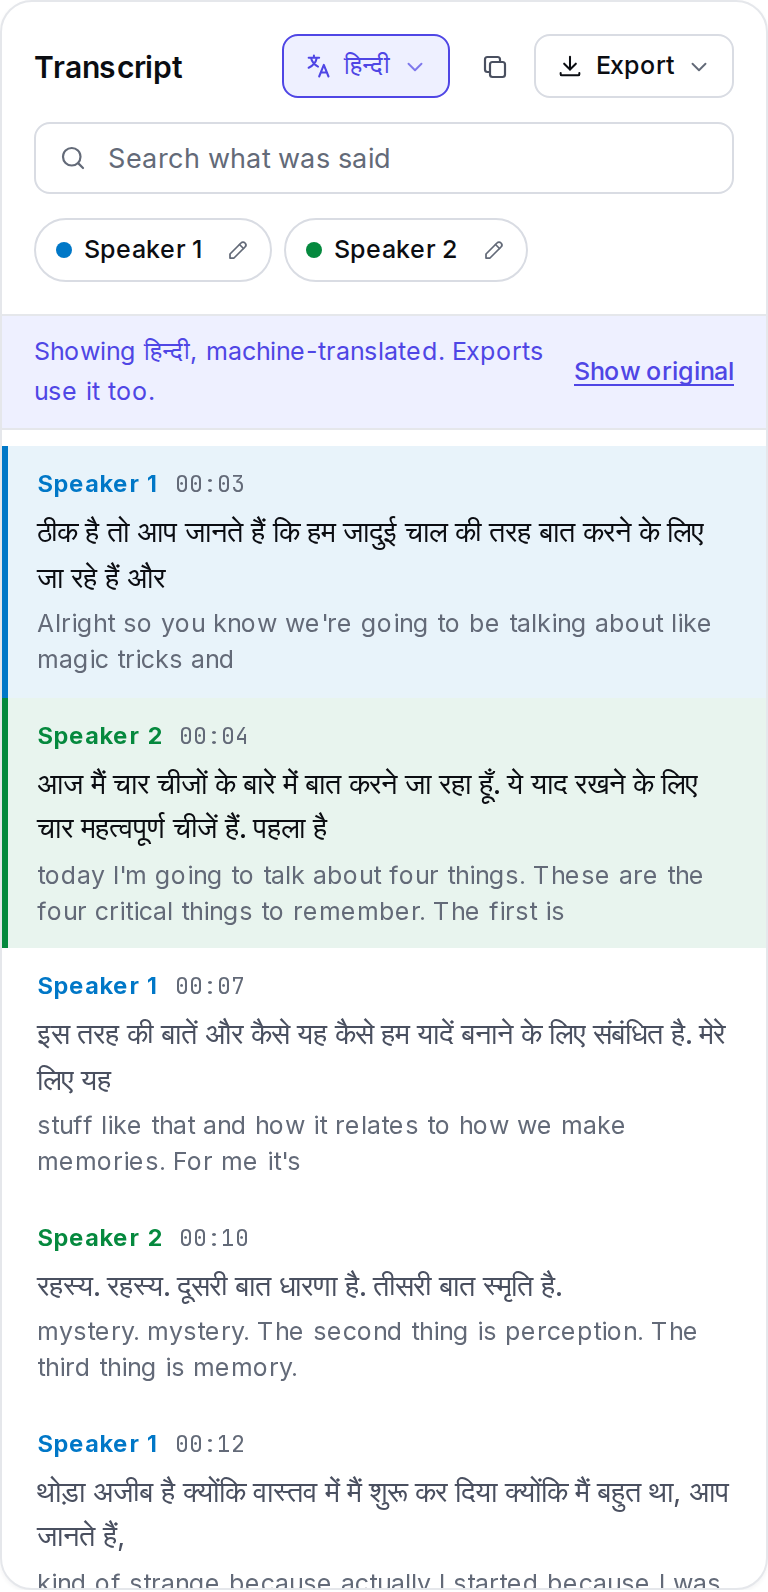
\includegraphics[width=\linewidth]{ui_transcript.png}\\[0.5mm]
\footnotesize (a) Transcript, read in Hindi
\end{minipage}\hfill
\begin{minipage}[b]{0.745\textwidth}
\centering
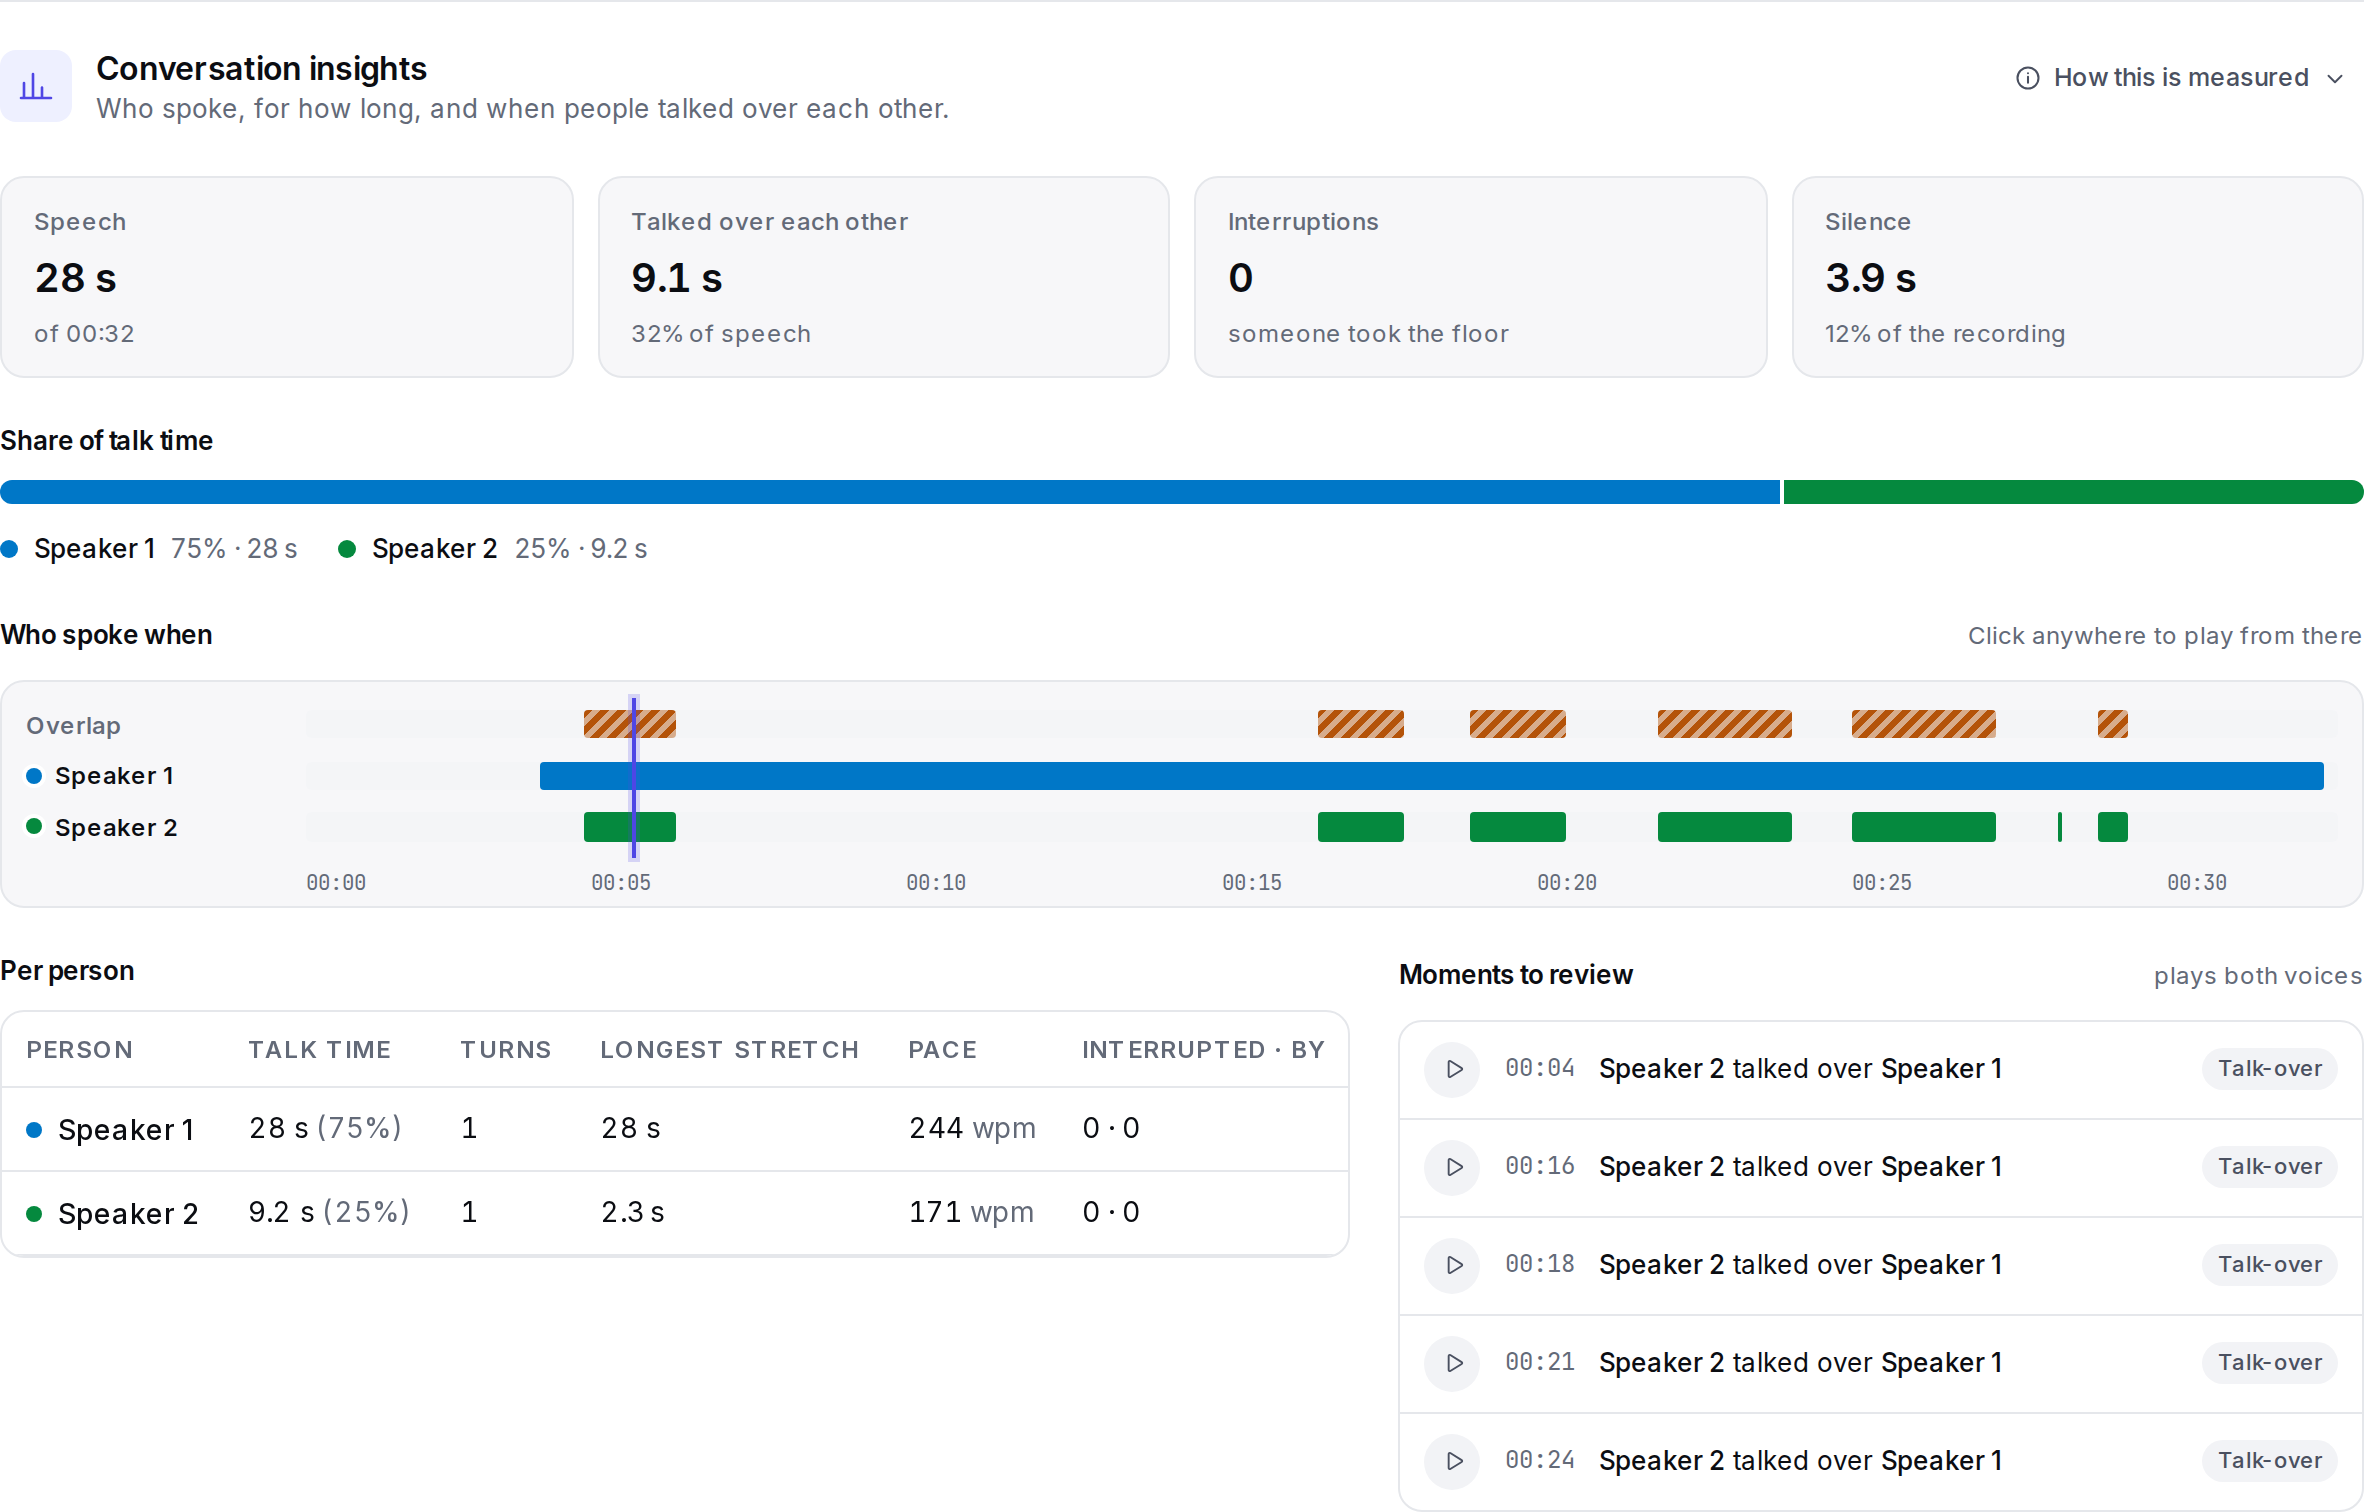
\includegraphics[width=\linewidth]{ui_insights.png}\\[0.5mm]
\footnotesize (b) Conversation insights
\end{minipage}
\caption{Conversation understanding in the production interface (live-site capture, AMI meeting ES2002a). (a) The merged transcript follows playback---during overlap both speakers' lines are highlighted---and is shown machine-translated into Hindi with the words as spoken beneath each line; selecting a line plays that person's separated voice. (b) Talk share, a who-spoke-when timeline with overlap regions, per-person statistics and moments to review, all from face-anchored diarization.}
\label{fig:conversation}
\end{figure*}

\subsection{Translated captions}
On request, every speaker's captions are translated by NLLB-200~\cite{nllb2024} (distilled 1.3B, pretrained, used as released under its non-commercial licence) through CTranslate2~\cite{ctranslate2} with 8-bit weights, the inference engine the recognizer already uses, so translation adds a model but no runtime dependency. Each caption segment is translated as one sentence and keeps its timing; word timings are dropped, since translation reorders words. The transcript, the player's caption and every export then read in the chosen language, with the original beneath each line (Fig.~\ref{fig:conversation}a). Forty target languages are offered, 18 of them scheduled languages of India, including four the recognizer cannot transcribe at all---Odia, Maithili, Kashmiri and Manipuri---so a meeting held in Kannada can be read in Odia. Every candidate target was screened by translating test sentences: Santali and Konkani produced SentencePiece unknown marks and untranslated English with the released model and are not offered, and the worker rejects any translation in which more than a fifth of the segments contain unknown marks. On the workstation, 100 caption segments translate in 0.7\,s once the model is loaded (4.7\,s, once per worker process). Translation quality is NLLB's own~\cite{nllb2024} and was not measured on this system.

\subsection{Summaries grounded in the transcript}
A summary---overview, key points, decisions and action items with owner and deadline---is written on request by Qwen2.5-7B-Instruct~\cite{qwen2025} (4-bit) served by Ollama~\cite{ollama} on the same GPU; nothing leaves the machine. Language models produce fluent text that is not always supported by their input; on the first trial, the model's overview said a speaker had lost weight, which nothing in the transcript states. We therefore require attribution in the spirit of citation-generation work~\cite{gao2023alce}: the prompt shows each line as \texttt{[L12 03:41 S2 Priya] text}, the answer is constrained to a JSON schema with bounded lists, and \emph{every} item, the overview included, must list the line ids it rests on. An item is kept only if at least one cited id is a real line, and an action item's owner must be one of the speakers or none. The page shows each item with play buttons for its cited lines, so the evidence is one click away. Long transcripts are summarised in parts of 220 lines; a part the model cannot answer within its token budget is halved, down to 30 lines.

\begin{table}[t]
\centering
\caption{Summaries of 30 AMI meetings from AMI's own speaker-attributed transcripts, against the action items and decisions AMI's annotators wrote. Lexical matching; a floor.}
\label{tab:summary}
\footnotesize
\setlength{\tabcolsep}{4pt}
\begin{tabular}{@{}lr@{}}
\toprule
Measure (30 meetings) & Value \\
\midrule
Meetings summarised / failed & 30 / 0 \\
Items citing no real line (dropped) & 0 of 314 \\
Action items P / R / F1 & 0.29 / 0.40 / 0.34 \\
\quad written / annotated / matched & 95 / 70 / 28 \\
Owner right (matched, role named) & 15 / 26 (58\%) \\
Decisions P / R / F1 & 0.00 / 0.00 / 0.00 \\
\quad written / annotated & 11 / 90 \\
Median time per meeting & 8.5\,s \\
\bottomrule
\end{tabular}

\end{table}

AMI's annotators recorded, for every scenario meeting, the actions agreed and the decisions taken, naming owners by role. We summarised each of the 30 meetings' \emph{whole} transcripts as AMI annotated them, with speakers named by role, and matched written items to annotated ones lexically (content words with role names removed, Dice overlap $\ge 0.35$, one-to-one), which undercounts paraphrases. This measures the summariser given a correctly attributed transcript; the separation's own errors are not compounded. Table~\ref{tab:summary} gives the result. Every meeting was summarised and no item had to be dropped for citing nothing real. Action items were found at a useful rate (recall 0.40, precision 0.29), and the owner was right for 15 of the 26 matched items that name a role (58\%; four roles, chance 25\%)---for example, the model's ``Review the user requirement specification'', owned by the Marketing Expert, against the annotators' ``The marketing expert will look at user requirement specifications'' (TS3005a). Many unmatched items are activities inside the meeting, such as AMI's warm-up exercise of drawing an animal, that annotators did not record as actions. Decisions were not found: the model wrote 11 against 90 annotated, and none matched. A median meeting took 8.5\,s.

\subsection{Shareable clips with burned-in captions}
People share moments, and video posted to feeds autoplays muted. An export can therefore be a clip---set by times, by the current playback position, or from transcript lines, where a second line stretches the clip---and can carry the captions in the picture, as spoken or in any translated language. Captions are written as ASS and drawn by ffmpeg's libass, which shapes Indic scripts with HarfBuzz; with several speakers each line leads with the name in that speaker's colour, and overlapping lines stack. A single-speaker export carries that speaker's captions only, matching its audio. Cutting or drawing requires re-encoding; the whole recording without captions is still a remux. In the end-to-end test, a 12\,s clip with Hindi captions was ready for download 4.3\,s after it was requested.


% ============================================================================
\section{Lessons from End-to-End Validation}
\label{sec:lessons}
% ============================================================================

Unit and integration tests passed throughout, yet the first browser-driven end-to-end test (sign in, upload, process, play, captions) against the production stack failed in ways no lower-level test could reach. Table~\ref{tab:defects} lists the defects it exposed, all now fixed and guarded by tests. They share a cause: in development every package was installed in one environment and ran as one user, and the reference pipeline's output had only ever been consumed by tests, while the player had only ever consumed mock output.

\begin{table}[t]
\centering
\caption{Defects exposed only by end-to-end testing}
\label{tab:defects}
\footnotesize
\setlength{\tabcolsep}{3pt}
\begin{tabular}{@{}>{\raggedright\arraybackslash}p{0.53\columnwidth}>{\raggedright\arraybackslash}p{0.41\columnwidth}@{}}
\toprule
Defect & Visible symptom \\
\midrule
API container user could not read the identity-provider key & every signed-in request failed (HTTP 500) \\
API imported worker packages absent from its image & uploads accepted, never processed \\
Presigned URLs signed for the internal storage host & uploads unreachable from browsers \\
Extractor fell back to CPU when \texttt{nvidia-smi} was off the service \texttt{PATH} & device-mismatch crash \\
Real manifest lacked the original-mix track and video & player failed to load \\
Caption JSON in a shape the player silently ignored & captions generated but never shown \\
Progress reported as a percentage, scaled by 100 again & bar full at the first update \\
Auth state read before session restore & ``401'' on opening a saved project \\
Concurrent first requests of a new account inserted the same user & language list empty after sign-up (HTTP 500) \\
Pace divided caption words by diarized talk time & a speaker at 412 words per minute \\
Longest turn spanned the other person's continuous speech & longest turn exceeding total talk time \\
Translation text kept while the next language loaded & Hindi shown under the name ``Odia'' \\
\bottomrule
\end{tabular}
\end{table}

Two practices proved decisive. Measuring rather than assuming offsets and identities (Eq.~\eqref{eq:lag}; the AMI camera mapping) prevented silent misalignment that would otherwise have surfaced as poor quality with no visible cause. And testing the deployed artefact through a real browser found more defects in one session than all earlier testing combined.

The corollary held for a path no test exercised. Video export had passed its unit tests but had never run in production, and building clips on it exposed three faults, each fatal on its own: the renderer read a source file that packaging never writes, so every video export would have degraded to audio; the rendered file was never uploaded, while the download link signed an object-store key that did not exist; and the download was a plain link to an authenticated route, which a browser navigates to without the bearer token. Operations taught a last lesson. The workstation's guest file system lives in a growable virtual disk on a host drive; downloading an 11\,GB model filled that drive, the guest file system went read-only, and the site was down until space was freed. On one machine every service shares fate with the disk, and free space has to be checked on the host, not inside the guest.

% ============================================================================
\section{Discussion}
\label{sec:discussion}
% ============================================================================

\textbf{Why the deployed model is not SEAVE.} SEAVE's audio-visual checkpoints were trained on 118 speakers and lost robustness to rooms (Table~\ref{tab:product}); its best robust checkpoint, C3, is audio-only and conditions on an enrolment embedding that must first be mined from the recording by diarization. The placeholder motion-energy active-speaker detector carried no usable signal (Section~\ref{sec:baseline}), so binding voices to faces for SEAVE's visual path was not yet possible. AV-MossFormer2 couples face tracking with lip-conditioned extraction, removing both dependencies, and produced correct speaker identity on every synthetic test track. The switch is an engineering decision, not a claim that it is the better separator on the product condition, which remains unmeasured for it. On real meetings SEAVE found a narrower role than intended: self-enrolled from a person's visible stretches it can fill off-screen gaps, but it improved intelligibility only slightly and did not improve captions (Section~\ref{sec:amiav}).

\textbf{What the evaluation shows.} Two results are methodological. In-domain validation inverted the ranking of models on the deployed condition, and an evaluation condition built to match the product, with overlap verified rather than assumed, was needed to see it. And on real meetings the weakest link was not separation quality but attribution: a recognizer transcribes speech far below the level any separator, or even a close-talk microphone, leaves behind, so per-speaker captions need an explicit decision about whose word each is. Cross-track deduplication is a simple such decision that is safe under overlap; the gap to an oracle (78.1\% against 45.1\% saWER) shows how much a learned one could still gain. The visual cue added about 0.4\dB on VoxCeleb2 for SEAVE, a thin margin that should not be generalised. Finally, the face-bound transcript and an audio-only diarizer turned out to be complements rather than competitors: words are best attributed by the faces, boundaries and overlap by the diarizer, and naming the diarizer's turns by the faces (Eq.~\eqref{eq:anchor}) gets both without a reference.

% ============================================================================
\section{Limitations and Future Work}
\label{sec:limits}
% ============================================================================

\begin{itemize}
\item \textbf{The deployed extractor is pretrained.} AV-MossFormer2 is used as released in ClearerVoice-Studio~\cite{clearervoice}; we did not train it. Its training data is described only as large-scale open-source data, so overlap with VoxCeleb2 cannot be ruled out for Table~\ref{tab:moss}. AMI is not known to be in it, but this cannot be verified either.
\item \textbf{AMI-AV is one domain.} Four static close-up cameras in meeting rooms, with mostly one person speaking at a time; the 2$\times$2 tiling places faces at fixed positions; ten meetings are held out. Heavy overlap is covered only by three synthetic videos scored against a Whisper pseudo-reference. On the fitting meetings the audio-only diarization baseline is clearly better in cpWER.
\item \textbf{Product-condition speakers} come from Libri2Mix dev, which was also used, in different mixtures, to select SEAVE checkpoints; the comparison between models is fair, but absolute numbers may be optimistic.
\item \textbf{No perceptual study.} No listening test was run; STOI is the only intelligibility measure, and caption hallucination was not measured separately from WER.
\item \textbf{Visibility.} Speech while a face is untracked is not recovered (14.4\% of speech on AMI-AV), and every word, including one said off screen, is placed under some visible face. Audio-only uploads are refused.
\item \textbf{Scale.} One GPU worker processes one job at a time; long recordings fall back to Web Audio playback because HLS output is not yet produced by the real pipeline.
\item \textbf{Data lifecycle.} Account and project deletion currently only marks records; a purge job for stored media remains to be built, which matters for a system that stores faces and voices.
\item \textbf{Conversation insights} inherit the visibility limit: a label anchored to the wrong face moves talk time with it, and on the held-out meetings talk share was worse with face anchoring than with caption words (16.1 against 13.1 points, $n{=}10$). Interruptions are found with F1 0.21; they are offered as moments to review, not as counts to rely on.
\item \textbf{Summaries} were evaluated on AMI's own transcripts, i.e.\ with perfect attribution, by lexical matching; their quality on VisioVox's transcripts is not measured, decisions were not found, and output is English only. A citation shows which lines an item is about, not that it reads them faithfully.
\item \textbf{Translation} quality was not measured here, two listed Indian languages had to be withdrawn after screening, and the translation model's licence is non-commercial---adequate for this zero-cost academic deployment, not for a commercial one.
\end{itemize}
Future work follows directly: a learned active-speaker detector on the face tracks, which would both narrow the gap to oracle attribution and decide which off-screen words belong to no visible face; a reverberant audio-visual product condition with a same-input comparison against C3; listening tests; summaries scored end to end on separated meetings, with a decision-extraction step the current model lacks; and translation evaluated against Indian-language references.

% ============================================================================
\section{Conclusion}
% ============================================================================

VisioVox turns a video in which people talk over each other into switchable per-speaker audio with captions, synchronized in a browser, and runs at zero recurring cost on the workstation that trained its models. Along the way we measured that window-wise blind separation scrambles identity on 29.8\% of transitions in real meetings, that a reliability-gated TSE model trained with room simulation holds $+8.25$\dB on a verified-overlap reverberant condition, and that the checkpoint with the best in-domain score made audio worse on that condition. On 30 real meetings, the deployed extractor helps where it sees a face, but transcribing its per-speaker tracks captioned every face with most of the meeting; deduplicating words across tracks reduced the error from 110\% to 78\% on held-out meetings without losing overlapped speech. On that face-attributed transcript, naming a diarizer's turns by face doubled overlap detection and tripled interruption detection, captions became readable in 40 languages, and summaries cite the lines behind every item---each measured against AMI where a reference exists, with what did not work reported beside what did. The broader lesson is that a separation system is validated by the condition it will serve and by the artefact users will touch, not by the benchmark on which it was trained.

% Column break before reference 39, so the two columns of the last page balance.
\IEEEtriggeratref{39}
\bibliographystyle{IEEEtran}
\bibliography{references}

\end{document}
